%% TMLR manuscript (venue decision: arXiv -> TMLR)
\documentclass{article}

\usepackage{tmlr}
\usepackage{amsmath}
\usepackage{amssymb}
\usepackage{mathtools}
\usepackage{longtable,array}
\usepackage{booktabs}
\usepackage{siunitx}
\sisetup{round-mode=places, round-precision=1, table-number-alignment=center, group-separator={}}
\usepackage{newunicodechar}
\newunicodechar{Σ}{\ensuremath{\Sigma}}
\newunicodechar{σ}{\ensuremath{\sigma}}
\newunicodechar{δ}{\ensuremath{\delta}}
\newunicodechar{α}{\ensuremath{\alpha}}
\newunicodechar{Ω}{\ensuremath{\Omega}}
\newunicodechar{ε}{\ensuremath{\varepsilon}}
\newunicodechar{γ}{\ensuremath{\gamma}}
\newunicodechar{ρ}{\ensuremath{\rho}}
\newunicodechar{λ}{\ensuremath{\lambda}}
\newunicodechar{η}{\ensuremath{\eta}}
\newunicodechar{μ}{\ensuremath{\mu}}
\newunicodechar{κ}{\ensuremath{\kappa}}
\newunicodechar{ν}{\ensuremath{\nu}}
\newunicodechar{φ}{\ensuremath{\phi}}
\newunicodechar{Ψ}{\ensuremath{\Psi}}
\newunicodechar{Ξ}{\ensuremath{\Xi}}
\newunicodechar{Θ}{\ensuremath{\Theta}}

% TikZ and PGFPlots for figures
\usepackage{tikz}
\usepackage{pgfplots}
\pgfplotsset{compat=1.18}
\usetikzlibrary{patterns, positioning, arrows.meta, shapes.geometric, backgrounds, fit}

% Algorithm environments
\usepackage{algorithm}
\usepackage{algpseudocode}

% Misc
\usepackage{enumitem}
\usepackage{amsthm}
\providecommand{\Description}[1]{}

% Theorem-like environments (results are hard-numbered to match the blueprint;
% the conjecture is auto-numbered so \ref resolves correctly).
\theoremstyle{definition}
\newtheorem{conjecture}{Conjecture}

% Custom commands
\newcommand{\R}{\mathbb{R}}
\DeclareMathOperator{\Var}{Var}
\DeclareMathOperator{\Corr}{Corr}
\DeclareMathOperator{\argmax}{arg\,max}
\DeclareMathOperator{\CosSim}{CosSim}

% Okabe-Ito colorblind-safe palette
\definecolor{okabe-ito-orange}{RGB}{230,159,0}
\definecolor{okabe-ito-skyblue}{RGB}{86,180,233}
\definecolor{okabe-ito-bluishgreen}{RGB}{0,158,115}
\definecolor{okabe-ito-yellow}{RGB}{240,228,66}
\definecolor{okabe-ito-blue}{RGB}{0,114,178}
\definecolor{okabe-ito-vermillion}{RGB}{213,94,0}
\definecolor{okabe-ito-purple}{RGB}{204,121,167}
\definecolor{okabe-ito-black}{RGB}{0,0,0}
\colorlet{sigmacolor}{okabe-ito-vermillion}
\colorlet{targetcolor}{okabe-ito-bluishgreen}
\colorlet{signalcolor}{okabe-ito-blue}
\colorlet{probefill}{okabe-ito-yellow!30}
\colorlet{odecolor}{okabe-ito-purple}
\colorlet{evalcolor}{okabe-ito-skyblue}
\colorlet{depthcolor}{signalcolor!12}
\colorlet{breadthcolor}{gray!12}
\colorlet{frontiercolor}{gray!70}

\usepackage{hyperref}
\hypersetup{
  pdftitle={Compositional Generalization as a Threshold Phase Transition: Why Adaptive Curricula are Unnecessary for Asymptotic Recovery},
  pdfsubject={Machine Learning, Dynamical Systems},
  pdfkeywords={compositional generalization, threshold dynamics, bifurcation theory, phase transitions, curriculum learning, stability exchange}
}

\title{Compositional Generalization as a Threshold Phase Transition: Why Adaptive Curricula are Unnecessary for Asymptotic Recovery\thanks{This submission was prepared with the assistance of large language models used as general-purpose assistive tools.}}
\author{\name Basyirin Amsyar Basri \email 26001270@siswa.um.edu.my \\
        \addr Universiti Malaya}
\date{}

\begin{document}
\maketitle

\begin{abstract}
\textbf{Problem:} Neural sequence models trained to high in-distribution (ID) accuracy systematically suffer catastrophic collapses when evaluated on zero-shot out-of-distribution (OOD) compositional recombinations. While existing literature frequently treats this failure as an optimization defect to be mitigated through dynamic curriculum design, we propose that compositional generalization is fundamentally governed by a macroscopic dynamical bifurcation.

\textbf{Theory:} We formulate a two-variable phenomenological dynamical model over \emph{parametric depth} $\delta_A$ (empirical risk specialization) and \emph{schema coherence} $\sigma_A$ (modular representational reorganization). The model establishes that standard empirical risk minimization drives networks into an asymptotically stable, low-coherence equilibrium (the $\sigma$-trap, $E_S$). Escaping this trap requires crossing a critical threshold ratio ($R_0 > 1$) associated with a transcritical exchange of stability toward a high-coherence attractor ($E_C$). Crucially, the bifurcation topology reveals that entering the coherent basin is a \emph{threshold phase transition} rather than a path-dependent trajectory optimization problem: within the ODE model, once $R_0(t) > 1$, convergence to $E_C$ is governed by basin attraction regardless of scheduling complexity.

\textbf{Empirical Findings:} We evaluate these theoretical predictions through controlled experiments on a SCAN-style compositional benchmark (H-Bar):
\begin{enumerate}[nosep]
\item \emph{Asymptotic Stability vs.\ Grokking:} Extended-horizon training on the baseline for $20{,}000$ steps ($10\times$ standard duration, with and without weight decay) provides strong finite-horizon evidence that the $\sigma$-trap is a stable attractor: training loss saturates to $0.0186$ and ID accuracy reaches $98.7\%$, yet OOD accuracy remains arrested at $34.7\%$, demonstrating that compositional failure does not spontaneously grok.
\item \emph{The Threshold Law and Fixed-Weight Parity:} A static, non-adaptive fixed-weight compositional loss ($\lambda=1.0$) achieves asymptotic OOD recovery identical to complex adaptive $\sigma$-modulated curricula ($98.9 \pm 3.6\%$ vs.\ $98.9 \pm 2.4\%$, Welch $p = 0.99$, TOST-equivalent within $\pm 2.5\%$). This parity provides strong empirical support for the threshold theory: dynamic curriculum scheduling is unnecessary for asymptotic recovery once the critical parameter boundary is crossed on this benchmark.
\item \emph{Dynamical Rate-Ordering:} The bifurcation structure structurally predicts the observed ordering of transition latencies across intervention conditions ($\hat{\tau}_{\text{fixed}} \approx 148 < \hat{\tau}_{\text{mult}} \approx 340 < \hat{\tau}_{\text{add}} \approx 542$ steps), demonstrating that scheduling governs transient efficiency rather than asymptotic destination.
\item \emph{Measurement Diagnostics:} Training-time gradient alignment (GCA) fails prospectively due to initialization subspace artifacts, while representational-geometry alignment (RGA, via CKA) robustly tracks structural exposure ($p = 0.005$).
\end{enumerate}

\textbf{Conclusion:} By demonstrating that compositional learning is governed by a global threshold bifurcation rather than path-dependent curriculum optimization, this framework explains why static compositional supervision suffices for asymptotic recovery on H-Bar and provides explicit dynamical foundations for training-time representational transitions.
\end{abstract}


% ============================================================
\section{Introduction}\label{sec:introduction}
% ============================================================

The dissociation between in-distribution competence and compositional generalisation is a pervasive phenomenon across deep learning. Models trained to near-perfect accuracy on sequence-to-sequence benchmarks frequently fail when required to execute zero-shot recombinations of familiar primitives. \cite{lake2018generalizationwithoutsystematicity} demonstrated this on the SCAN benchmark, where recurrent networks achieved $>99\%$ on random splits but $<2\%$ on the add-primitive split. Similar failures are documented in COGS \citep{kim2020cogscompositionalgeneralizationchallenge} (96--99\% ID vs.\ 16--35\% OOD) and PCFG-SET \citep{hupkes2020compositionalitydecomposed} across Transformers and recurrent architectures.

A prominent paradigm in machine learning approaches this failure as a delicate optimization problem, seeking to engineer dynamic curriculum schedules, pacing functions, or adaptive learning rates to guide models into compositional solutions \citep{bengio2009curriculumlearning,kumar2010selfpacedlearning,jiang2022mutualexclusivity}. In this paper, we challenge this premise: we demonstrate that compositional recovery can be modeled not as a path-dependent trajectory optimization problem, but as a \textbf{topological threshold event}.

We formalise the macroscopic training dynamics through the interaction of two state variables:
\begin{itemize}[nosep]
\item \textbf{Parametric depth} $\delta_A(d,t) \in [0, \Delta(d,t)]$: the degree to which network parameters have specialised to minimise empirical task loss on the training distribution.
\item \textbf{Schema coherence} $\sigma_A(d,t) \in [0,1]$: the degree to which internal representations are organised around the generative compositional rules and operators of the domain.
\end{itemize}

Because standard empirical risk minimisation (ERM) penalises only task error, gradient updates drive rapid accumulation of parametric depth $\delta_A$ via surface heuristics without exerting direct pressure to form modular schemas ($\sigma_A$). Under standard training, the model system enters an asymptotically stable, low-coherence equilibrium ($E_S$ in Proposition~2) where in-distribution performance saturates while compositional generalisation remains permanently arrested. We term this state the \textbf{$\sigma$-trap}.

\paragraph*{The Threshold Law: Why adaptive curricula are unnecessary for asymptotic recovery.}
By analyzing the stability of the $(\delta_A, \sigma_A)$ dynamical system, we prove that escaping the $\sigma$-trap is governed by a transcritical bifurcation at a critical threshold parameter $R_0 = 1$ (Proposition~4). When auxiliary compositional pressure pushes $R_0(t) > 1$, the failure equilibrium $E_S$ loses stability ($\lambda_2 > 0$) and exchanges stability with the coherent attractor $E_C$. 

Crucially, because entering the basin of attraction of $E_C$ in the model is a global topological transition, asymptotic recovery does not require fine-grained, adaptive path control. Once the parameter boundary $R_0 > 1$ is crossed, the vector field forces convergence toward the coherent state. Consequently, complex state-dependent curriculum scheduling is unnecessary for asymptotic performance: a naive, static fixed-weight loss that crosses $R_0 > 1$ achieves the identical asymptotic destination.

\paragraph*{Epistemic framing.}
The dynamical model developed in Section~\ref{sec:core-framework} is \emph{phenomenological}: its differential equations describe macroscopic phase-space geometry rather than microscopic parameter steps derived from first-principles SGD. The correspondence between SGD trajectories and the ODE vector field is formalised explicitly as an unproven modelling conjecture (Conjecture~\ref{conj:sgd-ode}).

\paragraph*{Contributions.}
This paper establishes four central contributions:
\begin{enumerate}[nosep]
\item \textbf{A dynamical bifurcation theory of the $\sigma$-trap.}
  We formulate a two-variable ODE system ($\delta_A, \sigma_A$) exhibiting a stable surface-learning equilibrium $E_S$, a coherent equilibrium $E_C$, and a transcritical exchange of stability at $R_0 = 1$ (Section~\ref{sec:core-framework}, Propositions~2--4).
\item \textbf{Empirical validation of the threshold law via fixed-weight parity.}
  In a controlled four-arm experiment ($n = 15$ per arm, 2000 steps) on a SCAN-style compositional benchmark (H-Bar), baseline training reproduces the trap ($90.2\%$ ID vs.\ $45.9\%$ OOD). We demonstrate that a static fixed-weight compositional loss achieves statistically and practically identical asymptotic OOD accuracy to complex adaptive $\sigma$-curricula ($98.9\%$ vs.\ $98.9\%$, Welch $p = 0.99$, TOST-equivalent within $\pm 2.5\%$; Section~\ref{sec:empirical-validation}). Rather than representing an algorithmic failure, this parity supports the threshold law: adaptive curricula are unnecessary for asymptotic recovery once the stability boundary is crossed. Crucially, the ODE bifurcation structure structurally predicts the observed rate-ordering of transition latencies ($\hat{\tau}_{\text{fixed}} < \hat{\tau}_{\text{mult}} < \hat{\tau}_{\text{add}}$).
\item \textbf{Decisive separation of the $\sigma$-trap from algorithmic grokking.}
  Through an extended $20{,}000$-step training experiment ($10\times$ standard horizon) across three weight-decay regimes, we confirm that standard ERM remains permanently arrested at $34.7\%$ OOD without grokking, experimentally providing strong finite-horizon evidence that the $\sigma$-trap is a stable attractor.
\item \textbf{Measurement diagnostics and representation geometry.}
  We show that gradient-composition alignment (GCA) is masked by an initialisation subspace artifact, explaining why local gradient metrics do not prospectively lead global transitions. Conversely, representational-geometry alignment (RGA, via CKA) functions as a robust exposure tracker ($r = +0.125, p = 0.005$) reflecting structural reorganization.
\end{enumerate}

All mathematical definitions, proofs (Appendix~\ref{app:proofs}), and proxy formulations (Appendix~\ref{app:stage1_proxy}) are fully self-contained in this manuscript.

\noindent\rule{\linewidth}{0.4pt}

% ============================================================
\section{Related Work and Gap Analysis}\label{sec:related-work}
% ============================================================

We review four literatures that bear on compositional generalisation
failure. To our knowledge, none models schema coherence as a dynamical
variable with its own evolution equation, suppression mechanism, and
critical threshold; making that gap precise is the purpose of this
review.

\subsection{Compositional Generalisation and Intervention Baselines}\label{sec:compositional-generalisation}

The SCAN/COGS/CFQ/PCFG-SET benchmark family collectively documents that standard neural sequence models encode superficial statistical regularities rather than the generative compositional rules of the domain \citep{lake2018generalizationwithoutsystematicity,
kim2020cogscompositionalgeneralizationchallenge,hupkes2020compositionalitydecomposed,mondorf2026compositionalarc}.
A substantial literature has proposed algorithmic remedies: data augmentation via primitive substitution \citep{andreas2020goodenoughcompositionaldataaug}, mutual-exclusivity training \citep{jiang2022mutualexclusivity}, dual-process architectures \citep{noviello2025neuroscienceinspiredualprocess}, structural representability analyses \citep{bruns2025exploringcompositionalgeneralizationin}, dataset cartography \citep{swayamdipta2020datasetcartography}, and aggressive scaling \citep{redhardt2025}. 

While these methods improve lexical or in-distribution accuracy, standard empirical risk minimisation (ERM) without explicit compositional supervision consistently fails to induce zero-shot recombination. Standard interventions such as increasing weight decay, adding dropout, or extending training to large step counts do not reliably close this gap because gradient descent along the task loss continues to deepen superficial pattern-matching. Our framework models this persistent failure not as an optimization defect, but as an *attractor state* ($\sigma$-trap) in the macroscopic representation space, and provides a formal condition ($R_0 > 1$) for when compositional supervision destabilises this attractor.

\subsection{Grokking, Phase Transitions, and Singular Learning Theory}\label{sec:grokking}

Grokking --- the sudden emergence of generalisation long after training loss saturates \citep{power2022grokking,liu2022grokking} --- is the temporal counterpart of the $\sigma$-trap, but differs fundamentally in its dynamical structure and task domain. Microscopic accounts of grokking explain the transition through a lazy-to-rich feature-learning crossover \citep{kumar2023grokkingeffectivetheory}, a dimensional phase transition in gradient-field geometry \citep{wang2026grokkingdimensionalphase}, basin selection ranked by the local learning coefficient (LLC) in Singular Learning Theory \citep{cullen2026basinselectiongrokking}, or critical thresholds in the Hessian spectrum \citep{montanari2026}; loss-landscape geometry and sharpness probes can serve as early-warning indicators \citep{xu2026earlywarning,foret2021sharpnessawareminimization}.

The $\sigma$-trap framework differs from these accounts in three decisive respects:
\begin{enumerate}[nosep]
\item \textbf{Asymptotic stability vs.\ transient metastability.} In standard grokking on algorithmic tasks (e.g., modular arithmetic), the memorising regime is a *metastable* plateau: regularisation (such as weight decay) slowly alters the effective loss landscape, enabling an unguided, noise-driven escape after prolonged training ($10^4$--$10^5$ steps). In contrast, on compositional tasks under standard task loss, the $\sigma$-trap is an *asymptotically stable equilibrium* ($E_S$ in Proposition~2): gradient updates actively reinforce surface heuristics ($\dot{\delta}_A > 0, \dot{\sigma}_A < 0$ when $R_0 < 1$). The agent does not spontaneously escape through extended training; escape requires altering the vector field via compositional pressure ($R_0 > 1$).
\item \textbf{Transcritical bifurcation vs.\ saddle-node/annihilation.} While grokking is frequently conceptualised as a saddle-node bifurcation where the memorisation basin vanishes, the $\sigma$-trap undergoes a *transcritical bifurcation* (Proposition~4). The surface-learning state $\sigma_A = 0$ persists as a fixed point for all parameter values, but exchanges stability with the coherent branch $\sigma_A^*$ at $R_0 = 1$. The failure state is never physically annihilated; it is rendered unstable.
\item \textbf{Compositional specificity.} Grokking concerns delayed generalisation on uniform/i.i.d.\ validation splits. The $\sigma$-trap specifically models the dissociation where in-distribution validation accuracy reaches saturation ($\ge 90\%$) while zero-shot out-of-distribution recombination fails near-completely.
\end{enumerate}

\subsection{Representation and Feature-Learning Dynamics}\label{sec:repr-dynamics}

Accounts that relate generalisation to the geometry of learned
representations include sharpness of the loss landscape
\citep{foret2021sharpnessawareminimization}, sparse-subnetwork
selection \citep{frankle2019lotteryticket}, and shortcut learning ---
reliance on surface features rather than structure
\citep{geirhos2020shortcutlearning}. These describe properties of the
solution or the strategy it encodes; the $\sigma$-trap describes the
representational state produced by the competition between shortcut
exploitation and schema formation, and derives a threshold
($\sigma_{\text{critical}}$) for when that competition is resolved in
favour of compositional competence.

\subsection{Curriculum Interventions}\label{sec:curriculum}

Easy-to-hard curricula provide representational scaffolding
\citep{bengio2009curriculumlearning,kumar2010selfpacedlearning,
portelas2020automaticcurriculumlearningdeep,narvekar2020curriculumlearningreinforcementlearning},
with recent evidence that ordering alone yields no robust advantage on
deductive-reasoning benchmarks \citep{mordig2026rethinkingeasytohard};
meta-learning over procedurally generated tasks can induce task-specific
schemas that transfer poorly across domains
\citep{mondorf2026compositionalarc}. The $\sigma$-modulated curriculum
studied in this paper is not a new ordering method: it couples the
training objective to the model's own coherence state. The gate
experiment isolates the value of that coupling by comparing it against
a fixed-weight compositional-loss baseline that uses no coupling at all
(Section~\ref{sec:empirical-validation}).

\paragraph{Positioning.}
Existing accounts of compositional generalisation have characterised
the problem through task structure, representation geometry, shortcut
learning, scaling, curriculum design, or optimisation dynamics. We
introduce a complementary dynamical construct --- schema coherence ---
that explicitly represents the degree to which learned representations
support systematic recombination. The claim is not that compositional
generalisation involves a training transition, but that this transition
can be described by a low-coherence attractor with a critical threshold.
The distinguishing empirical signature is compositional-specific failure
conditional on matched in-distribution accuracy. Following the
competing-variable design of Section~\ref{sec:empirical-validation}, a
schema-coherence measure must predict compositional OOD behaviour beyond
in-distribution accuracy, training loss, parameter norm, and
loss-landscape geometry; the gate experiment reports the first such
checks --- a fixed-weight control and partial-correlation controls.

\noindent\rule{\linewidth}{0.4pt}

% ============================================================
\section{The \texorpdfstring{$\sigma$}{sigma}-Trap: A Two-Variable Dynamical Model}\label{sec:core-framework}
% ============================================================

We model the training dynamics of an agent on a compositional task with
two state variables: \textbf{parametric depth} $\delta_A(d,t)$ and
\textbf{schema coherence} $\sigma_A(d,t)$. The model is deliberately
\emph{phenomenological}: the equations below are posited as a compact
description of the behaviour observed in the gate experiment
(Section~\ref{sec:empirical-validation}), not derived from first
principles of gradient-based optimisation. The link between real SGD
trajectories and the model is an explicit, unproven assumption:

\begin{conjecture}[SGD--ODE mapping; modelling assumption]
\label{conj:sgd-ode}
For the architecture and training protocol of
Section~\ref{sec:empirical-validation}, there exist empirical
diagnostics --- parametric depth $\delta_A$ and schema coherence
$\sigma_A$ measured by the Stage-1 proxies (see Appendix~\ref{app:stage1_proxy}) --- whose evolution along SGD trajectories is well approximated,
in the scaling regime of the gate experiments, by the two-variable ODE
system (Eqs.~\eqref{eq:depth-ode} and \eqref{eq:sigma-ode}). The
conjecture licenses transferring the qualitative predictions of the ODE
analysis --- existence of a stable low-$\sigma_A$ equilibrium, the
$\sigma_{\text{critical}}$ crossing, and the Phase~2 inflection --- to
trained networks.
\end{conjecture}

\noindent\emph{Status.} Conjecture~1 is an assumption, not a result.
Nothing in this paper asserts that SGD itself instantiates the ODEs; the
ODEs are a phenomenological description. The mathematical results of
this section (Lemmas~1--2, Propositions~2--4) are theorems \emph{about
the ODE model} and remain valid whether or not the conjecture holds:
they are model-conditional, and no downstream result silently depends on
the conjecture being true. Empirical support is deferred to the gate
experiment (Section~\ref{sec:empirical-validation}), which detects the
Phase~2 entry signature in the $\sigma$-modulated arms; the conjecture
fails if the Stage-1 proxies fail \emph{simultaneously} --- i.e., if no
measured quantity tracks the modelled state, the ODE analysis has no
empirical counterpart. The gate results support the \emph{descriptive}
use of the model (the trap behaviour is reproduced) but provide no
evidence that measured $\sigma_A$ precedes OOD improvement (partial
correlation $\approx 0$; Section~\ref{sec:empirical-validation}). No
leading-indicator role may be attached to this conjecture.

\noindent In the two-variable core, $\alpha_A$ (attentional fidelity),
$\Omega_{SL}$ (shortcut-learning pressure), and $P_A$ (availability of
principled structure) enter as \emph{fixed or environmental inputs} ---
parameters of the core system, not state variables. This keeps the state space strictly
two-dimensional, $\mathcal{X} = [0, \Delta_{\max}] \times [0, 1]$.

\subsection{State Variables}\label{sec:state-variables}

\subsubsection{Parametric Depth \texorpdfstring{$\delta_A(d,t)$}{delta\_A(d,t)}}\label{sec:depth}

The structural complexity of the agent's internal representation of the
task domain $d$: the degree to which parameters have specialised to the
training distribution. Bounded above by the domain frontier
$\Delta(d,t)$:
\begin{equation}\label{eq:depth-bounds}
0 \leq \delta_A(d,t) \leq \Delta(d,t)
\end{equation}
\textbf{Relative depth:}
\begin{equation}\label{eq:relative-depth}
\delta_A^{\text{relative}}(d,t) = \frac{\delta_A(d,t)}{\Delta(d,t)} \in [0,1]
\end{equation}

\subsubsection{Schema Coherence \texorpdfstring{$\sigma_A(d,t)$}{sigma\_A(d,t)}}\label{sec:schema-coherence}

Schema coherence $\sigma_A(d,t) \in [0,1]$ quantifies the degree to
which the agent's representation has been restructured around the
compositional structure of the task --- the operators and recombination
rules that generate the distribution --- rather than surface statistics.
High $\sigma_A$ indicates that the representation encodes compositional
operators applicable beyond the training distribution; low $\sigma_A$
indicates memorisation of surface patterns that fail to transfer.

$\sigma_A$ is distinct from OOD accuracy in kind: it is a property of
the \emph{representation} (internal state), while OOD accuracy is a
property of \emph{behavioural output}; two agents can achieve identical
OOD accuracy through different mechanisms (memorisation vs.\ genuine
recombination), and only the latter exhibits high $\sigma_A$.
Operationally, $\sigma_A$ is measured at training time by the Stage-1
proxies --- gradient-composition alignment (GCA), representational-
geometry alignment (RGA), and augmentation consistency (AC) --- fused as
$\tilde{\sigma}_A$. Concretely, GCA computes the cosine alignment
between per-step parameter gradients and a compositional reference
direction derived from the task's recombination rules; RGA scores the
similarity (CKA-style) between the representational geometry of
training inputs and of their compositional recombinations; and AC
measures prediction consistency under primitive-substitution
augmentation. The three signals are normalised to $[0,1]$ and combined
as a weighted average; the gate experiment used the two-signal GCA+RGA
sub-fusion, and the full three-signal protocol, its mathematical definitions,
two-stage calibration, and estimation bounds are given in Appendix~\ref{app:stage1_proxy}.
Throughout, $\sigma_A$ denotes the theoretical construct, $\tilde{\sigma}_A$
its training-time estimate, and $\hat{\sigma}_A$ the post-hoc diagnostic;
the construct is not directly observable, and the estimates are
imperfect (Section~\ref{sec:empirical-validation}). Operationally, in the present experimental evaluation, $\sigma_A$ is tracked via representation geometry (RGA) and post-hoc diagnostics ($\hat{\sigma}_A$), whereas parametric depth $\delta_A$ is modeled as a latent variable reflecting empirical risk specialisation on the training loss. The present empirical tests therefore focus directly on the $\sigma_A$ dynamical dimension; future work will operationalize layer-wise weight-norm and representation-rank probes for $\delta_A$. The Stage-2 diagnostic
$\hat{\sigma}_A = \text{Acc}_{\text{OOD}}/\text{Acc}_{\text{ID}}$ is
defined from the same accuracies it describes and is used in this paper
\emph{post-hoc} only, as a descriptive summary of the measured gap ---
never as a training signal and never as evidence for a causal
relationship (Section~\ref{sec:empirical-validation}).

\subsection{Mastery and Decay}\label{sec:mastery-set}

The \textbf{mastery set} collects the domains in which the agent has
both sufficient depth and sufficient schema coherence:
\begin{equation}\label{eq:mastery-set}
M_A(t) = \{d \in D : \delta_A(d,t) > \theta_{\delta} \cdot \Delta(d,t) \text{ AND } \sigma_A(d,t) > \theta_{\sigma}\}
\end{equation}
with $\theta_{\delta}, \theta_{\sigma} \in [0,1]$ the depth and
coherence mastery thresholds (Appendix~\ref{app:notation}).

Learned structure decays in the absence of reinforcement, while schema coherence provides structural protection against parametric forgetting:
\begin{equation}\label{eq:effective-decay}
\mu_c^{\text{eff}}(d,t) = \mu_c \cdot (1 - \gamma_\sigma \cdot \sigma_A(d,t))
\end{equation}
\begin{equation}\label{eq:depth-decay}
\dot{\delta}_A(d,t)\big|_{\text{decay}} = -\mu_c \cdot (1 - \gamma_\sigma \cdot \sigma_A(d,t)) \cdot \delta_A(d,t) \cdot (1 - r_A(d,t))
\end{equation}
where $\mu_c > 0$ is the base parametric decay rate.

\subsection{Evolution Equations and Environmental Coupling}\label{sec:evolution-equations}

\subsubsection{Parametric Depth ODE}
\begin{equation}\label{eq:depth-ode}
\dot{\delta}_A(d,t) = f_{\text{learn}}(d,t) \cdot \eta(d,t) \cdot T_A(d,t) - \mu_c \cdot (1 - \gamma_\sigma \cdot \sigma_A(d,t)) \cdot \delta_A(d,t) \cdot (1 - r_A(d,t))
\end{equation}
with learning efficiency in Gompertz form:
\begin{equation}\label{eq:gompertz}
\eta(d,t) = \eta_{\text{max}} \cdot \exp(-a \cdot \exp(-b \cdot \delta_A^{\text{relative}}(d,t)))
\end{equation}
where $\eta_{\max}$ is the maximal learning efficiency and
$a, b > 0$ shape the Gompertz curve (Appendix~\ref{app:notation}).
Depth grows when learning efficiency and time-on-task are large, and
decays when schema coherence is low (little protection from forgetting).

\noindent\textit{Choice of Gompertz formulation.} The Gompertz function $\eta(\delta^{\text{rel}}) = \eta_{\max} \exp(-a \exp(-b \delta^{\text{rel}}))$ was selected over a standard logistic curve because learning efficiency exhibits \textit{asymmetric saturation}. A logistic curve is symmetric around its 50\% inflection point. However, mastery trajectories in both human and artificial learning demonstrate that early acquisition accelerates quickly once initial representations form, but late-stage mastery of edge-case recombinations faces severe, exponentially diminishing returns. The Gompertz curve naturally reflects this asymmetry: its inflection occurs early at $\delta^{\text{rel}} = \frac{\ln a}{b}$, followed by a long, slow approach to $\eta_{\max}$, accurately modeling the asymptotic difficulty of depth specialization.

\subsubsection{Schema Coherence ODE and Loss Coupling}
\begin{equation}\label{eq:sigma-ode}
\dot{\sigma}_A(d,t) = \sigma_A(d,t) \cdot \bigl[ \rho \cdot P_A(d,t) \cdot \alpha_A \cdot (1 - \gamma_{\sigma} \cdot \sigma_A(d,t)) - \epsilon_{\sigma} \cdot \Omega_{SL}(d,t) \bigr]
\end{equation}
where $\rho$ is the schema growth rate, $P_A(d,t)$ the availability of
principled structure, $\alpha_A$ the attentional fidelity (a fixed
parameter of the core system), $\gamma_\sigma$ the saturation coefficient, $\epsilon_\sigma$
the shortcut-suppression coefficient, and $\Omega_{SL}(d,t)$ the
shortcut-learning pressure.

\noindent\textit{Environmental loss coupling.} The quantities $\Omega_{SL}(d,t)$ and $P_A(d,t)$ are external forcing functions governed by the training loss composition $\mathcal{L}(t) = \mathcal{L}_{\text{task}}(t) + \lambda(t) \mathcal{L}_{\text{comp}}(t)$, where $\lambda(t)$ is the effective compositional supervision weight:
\begin{equation}\label{eq:loss-coupling}
\Omega_{SL}(t) = \frac{\Omega_0}{1 + \kappa_\lambda \lambda(t)}, \qquad P_A(t) = P_0 + \kappa_p \lambda(t)
\end{equation}
where $\Omega_0$ is baseline shortcut pressure and $\kappa_\lambda, \kappa_p > 0$ couple supervision to the dynamical parameters. Standard training ($\lambda(t) \equiv 0$) keeps shortcut pressure high ($\Omega_{SL} = \Omega_0$) and principled structure low ($P_A = P_0$), locking $R_0 < 1$. Compositional supervision ($\lambda(t) > 0$) suppresses shortcut exploitation and amplifies principled structure, driving $R_0(t) > 1$.

\noindent\textit{Intuition.} The $\sigma_A$ ODE has an autocatalytic
structure: growth is proportional to current coherence ($\sigma_A$)
times the net driving force in the bracket. The bracket captures whether
principled understanding builds faster than shortcut pressure erodes it.
When $\sigma_A$ is near zero, growth stalls entirely because the
$\sigma_A$ factor suppresses the whole right-hand side. This creates the
critical bifurcation at the heart of the model: below a threshold, the
$\sigma_A = 0$ state is stable and self-perpetuating --- the
$\sigma$-trap; above it, coherence grows toward a positive equilibrium.

\subsection{Mathematical Foundations}\label{sec:math-foundations}

The coupled system (Eqs.~\eqref{eq:depth-ode} and \eqref{eq:sigma-ode})
is a two-dimensional nonlinear ODE on the state
$\mathbf{x}_A(t) = (\delta_A(t), \sigma_A(t)) \in \mathcal{X}$, where
\begin{equation}\label{eq:state-vector}
\mathbf{x}_A(t) = (\delta_A(t), \sigma_A(t))^{\mathsf{T}},
\qquad
\mathcal{X} = [0, \Delta_{\max}] \times [0, 1].
\end{equation}
We suppress the domain index $d$ throughout this section.

\textbf{Lemma 1 (Local Existence and Uniqueness).}
\emph{For any initial condition $\mathbf{x}_A(0) \in \text{int}(\mathcal{X})$,
the system admits a unique solution $\mathbf{x}_A(t)$ on a maximal
interval $[0, T_{\max})$ with $T_{\max} > 0$.}

\emph{Proof.} In Appendix~\ref{app:proofs}.

\textbf{Lemma 2 (Forward Invariance and Boundedness).}
% relabelled from Prop 3.2
\emph{$\mathcal{X}$ is forward-invariant under the clamped dynamics
(the upper bound $\sigma_A = 1$ is enforced by the solver's boundary
clipping; see the proof in Appendix~\ref{app:proofs}): if
$\mathbf{x}_A(0) \in \mathcal{X}$, then $\mathbf{x}_A(t) \in \mathcal{X}$
for all $t \in [0, T_{\max})$. If $\Delta_{\max} < \infty$, then
$T_{\max} = \infty$ (global existence).}

\emph{Proof.} In Appendix~\ref{app:proofs}.

\textbf{Proposition 2 (Equilibria of the Two-Variable Core).}
% relabelled from Prop 3.4
\emph{For constant frontier $\Delta$ and fixed parameters, the system
admits exactly three equilibrium classes:}
\begin{enumerate}[nosep]
\item \textbf{Trivial equilibrium} $E_0 = (0, 0)$: no knowledge
  acquired. Exists iff the effective training input vanishes
  ($f_{\text{learn}} \cdot T_A = 0$): under the Gompertz form
  $\eta(0) = \eta_{\max} e^{-a} > 0$, so $\dot{\delta}_A > 0$ at
  $\delta_A = 0$ whenever training input is nonzero (consistent with
  Lemma~2's boundary check).
\item \textbf{Surface-learning equilibrium}
  $E_S = (\delta_S^*, 0)$: depth acquired but $\sigma_A = 0$. Exists
  when shortcut-learning pressure is high ($\epsilon_\sigma \Omega_{SL} >
  \rho P_A \alpha_A$). This is the $\sigma$-trap.
\item \textbf{Schema-coherent equilibrium}
  $E_C = (\delta_C^*, \sigma_C^*)$ with $\sigma_C^* > 0$: both depth and
  coherence positive; exists and is stable iff $R_0 > 1$, i.e.\ iff the
  \emph{fixed} parameter $\alpha_A > \epsilon_\sigma \Omega_{SL} /
  (\rho P_A)$ (a condition on the parameter, not on its dynamics).
\end{enumerate}

\emph{Proof.} In Appendix~\ref{app:proofs}.

\textbf{Proposition 3 (Low-$\sigma$ Trap: Global Stability).}
% relabelled from Thm 4.1; model-conditional per the P05 relabel plan
\emph{If $R_0 < 1$ --- i.e.\ the shortcut pressure dominates,
$\epsilon_\sigma \Omega_{SL} > \rho P_A \alpha_A$ --- then, under the
dynamics of \eqref{eq:sigma-ode} alone, $\dot{\sigma}_A < 0$ for all
$\sigma_A \in (0,1]$, and the schema-free state $\sigma_A = 0$ is
\emph{globally} attracting on $[0,1]$: the model's low-coherence state
is a stable trap. This is a statement about the model, not about real
SGD; whether SGD enters this regime is the subject of
Conjecture~\ref{conj:sgd-ode}.}

\emph{Proof.} In Appendix~\ref{app:proofs}.

\textbf{Proposition 4 ($\sigma_{\text{critical}}$ and the Transcritical
Bifurcation).}
% relabelled from Prop 4.1; main theorem of the narrow paper
\emph{Define the basic schema growth ratio
\begin{equation}
R_0 = \frac{\rho \cdot P_A \cdot \alpha_A}{\epsilon_\sigma \cdot \Omega_{SL}}.
\end{equation}
The Phase~1$\to$2 transition threshold is
\begin{equation}\label{eq:sigma-critical}
\sigma_{\text{critical}} = \frac{1}{\gamma_\sigma} \cdot \left(1 - R_0^{-1}\right).
\end{equation}
When $R_0 > 1$, the schema-free equilibrium $\sigma_A = 0$ becomes
unstable and the schema-coherent equilibrium emerges via a
\emph{transcritical} bifurcation at $R_0 = 1$.}

\emph{Proof.} In Appendix~\ref{app:proofs}.

\noindent\emph{Intuition and interpretation of the threshold.} The parameter $R_0$ is borrowed from epidemiology: when $R_0 > 1$, one unit of schema coherence generates more than one unit of additional coherence --- understanding snowballs. When $R_0 < 1$, schemas die out and the agent remains trapped in $E_S$. Standard training maintains $R_0 < 1$ by inflating shortcut-learning pressure $\Omega_{SL}$ (Proposition~4). Notice that when $R_0 < 1$, Eq.~\eqref{eq:sigma-critical} yields $\sigma_{\text{critical}} < 0$. Because $\sigma_A \in [0, 1]$, a negative threshold lies strictly outside the physical state space, formally indicating that *no crossing is possible* and the schema-free state $\sigma_A = 0$ is unconditionally stable across the entire interval $[0, 1]$ (Proposition~3). Interventions that introduce compositional supervision lower effective shortcut pressure $\Omega_{SL}$, raising $R_0$ above $1$ and shifting $\sigma_{\text{critical}}$ into the accessible domain $(0, 1]$.

\noindent\emph{Dual-coupling calibration of $\lambda_{\text{crit}}$.} Under the loss-coupling formulation of Eq.~\eqref{eq:loss-coupling}, auxiliary compositional loss simultaneously suppresses shortcut pressure ($\Omega_{SL}(\lambda) = \Omega_0 / (1 + \kappa_\lambda \lambda)$) and amplifies structure availability ($P_A(\lambda) = P_0 + \kappa_p \lambda$). Setting $R_0(\lambda) = \frac{\rho (P_0 + \kappa_p \lambda) \alpha_A}{\epsilon_\sigma \Omega_0 / (1 + \kappa_\lambda \lambda)} = 1$ with the canonical simulation parameters of Table~\ref{tab:ode-params} yields the quadratic equation $3\lambda^2 + 1.9\lambda - 0.8 = 0$, whose positive root is $\lambda_{\text{crit}} \approx 0.289$. Thus, the experimental choice of nominal $\lambda_0 = 1.0$ places the fixed-weight arm deeply into the supercritical regime ($R_0(\lambda_0) \approx 5.1 > 1$), explaining why static fixed supervision immediately triggers Phase~2 recovery without fine-tuning.

\noindent\emph{Parameter sensitivity and topological robustness.} While the exact quantitative numerical timing $\hat{\tau}$ depends on optimization hyperparameters (learning rate, batch size), the \textit{qualitative bifurcation structure} of the system is topologically invariant to parameter variations. The local Jacobian eigenvalues at $E_S$ and $E_C$ depend strictly on the sign of $R_0 - 1$ (Appendix~\ref{app:stability}). Scaling any positive parameter $(\rho, P_0, \alpha_A, \epsilon_\sigma, \Omega_0, \gamma_\sigma)$ by $\pm 50\%$ alters only the location of the critical threshold $\lambda_{\text{crit}}$, leaving the existence of the $\sigma$-trap at $R_0 < 1$ and the transcritical exchange of stability at $R_0 = 1$ mathematically intact. Furthermore, the physical meaning of the $\sigma_A = 0$ branch persisting at $R_0 > 1$ is that a completely schema-free initialization is an unstable saddle point: while a hypothetical zero-state has $\dot{\sigma}_A = 0$ under continuous flow, any non-zero initial schema component $\sigma_A(0) > 0$ or stochastic gradient perturbation triggers dynamic repulsion toward $E_C$.

\noindent\emph{Against a purely logistic reading: Phase-space geometry vs.\ curve fitting.} On a single isolated OOD trajectory, the observable accuracy curve can resemble an S-shaped sigmoid, prompting the question of why a two-variable dynamical system is required rather than a standard empirical curve fit (e.g., a three-parameter logistic or Gompertz function). We address this on both theoretical and empirical grounds:
\begin{enumerate}[nosep]
\item \textbf{Theoretical content:} A fitted sigmoid is a descriptive parameterisation of monotonic growth from any starting point; it has no phase-space content. It cannot represent the persistent stability of the baseline failure state $E_S$ (where $\dot{\sigma}_A < 0$), the unstable separator, the threshold parameter $R_0$, or the transcritical exchange of stability at $R_0 = 1$ (Proposition~4). The model's predictions concern that phase-space geometry and bifurcation structure, not merely the geometric shape of an isolated curve.
\item \textbf{Empirical model comparison:} Formally fitting both 3-parameter Logistic and Gompertz models to the experimental OOD trajectories reveals that no single S-curve family universally describes the data across conditions. On the fixed-weight arm, the asymmetric Gompertz model substantially outperforms the symmetric logistic curve ($\Delta\text{AIC} \approx 50$), reflecting rapid takeoff followed by a long saturation tail. Conversely, on the additive and multiplicative curriculum arms, the logistic curve provides a superior fit ($\Delta\text{AIC} \approx 19\text{--}22$), while on the flat baseline arm both models tie. The ODE system unifies these divergent trajectory shapes under a single structural mechanism governed by effective compositional pressure.
\end{enumerate}

\noindent\emph{Bifurcation parameter and nonautonomous quasi-static dynamics.} In actual neural network training, $\lambda(t)$, $\Omega_{SL}(t)$, and $P_A(t)$ evolve over training time, making the true continuous system nonautonomous. Our bifurcation analysis operates under a standard \emph{quasi-static approximation}: because the learning rate $\eta \sim 10^{-3}$ induces slow parameter evolution relative to per-step activation dynamics, the rate of change of the effective schedule $\dot{\lambda}(t)$ satisfies an adiabatic timescale separation $|\dot{\lambda}(t)/\lambda(t)| \ll 1/\tau_{\text{relax}}$, ensuring that the instantaneous autonomous phase portrait and Jacobian eigenvalues $\lambda_2(t)$ dictate the qualitative vector field and stability transitions. Standard cross-entropy maintains high $\Omega_{SL}(t)$ (keeping $R_0(t) < 1$), while auxiliary compositional supervision reduces $\Omega_{SL}(t)$. Consequently, Phase~2 entry ($\sigma_A > \sigma_{\text{critical}}(t)$) is enabled as compositional supervision pushes $R_0(t) > 1$, transitioning $\sigma_{\text{critical}}(t)$ into the accessible interval $(0, 1]$.
Figure~\ref{fig:bifurcation} illustrates the bifurcation structure and the $(\delta_A, \sigma_A)$ phase portrait with the three equilibria.

\begin{figure}[htbp]
\centering
\resizebox{0.95\textwidth}{!}{\usetikzlibrary{positioning, arrows.meta, patterns, backgrounds, fit}

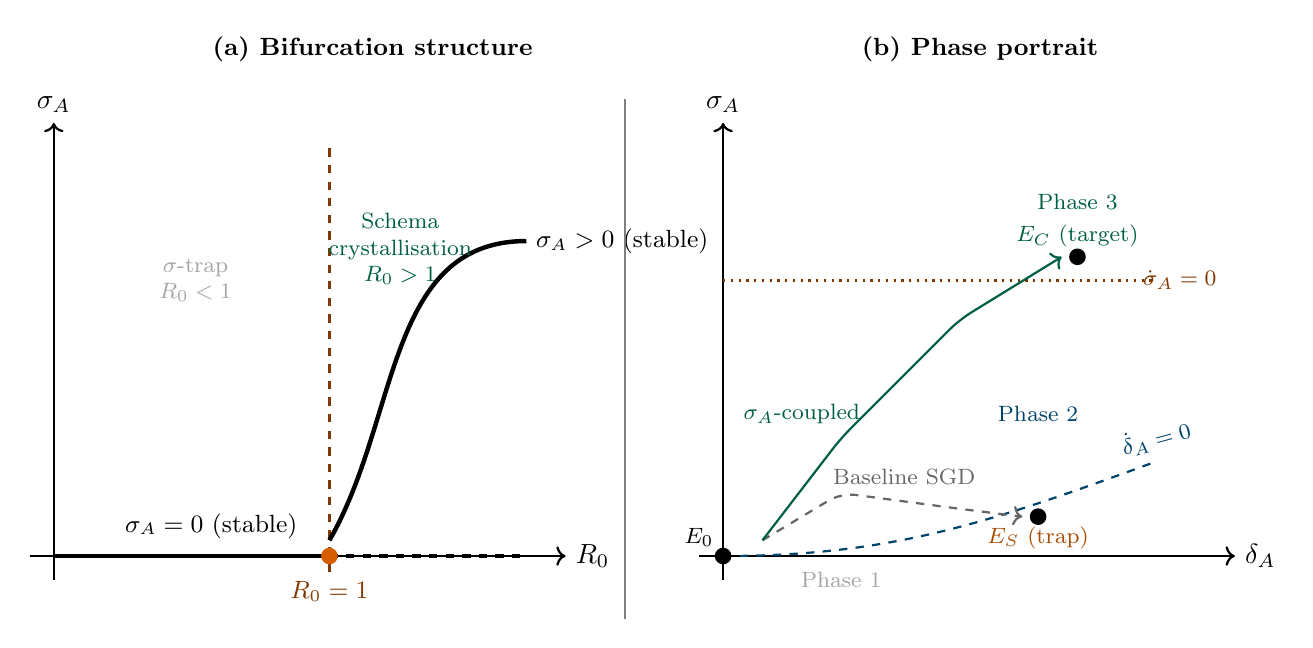
\begin{tikzpicture}[font=\sffamily]

    % ===== PANEL (a): Bifurcation Diagram =====
    \begin{scope}[local bounding box=bifurcation]
        \draw[->, thick] (-0.3, 0) -- (6.5, 0) node[right] {$R_0$};
        \draw[->, thick] (0, -0.3) -- (0, 5.5) node[above] {$\sigma_A$};

        % R_0 = 1 line
        \draw[dashed, thick, sigmacolor!60!black] (3.5, -0.2) -- (3.5, 5.2);
        \node[below, font=\small, text=sigmacolor!60!black] at (3.5, -0.2) {$R_0 = 1$};

        % Stable equilibrium branch (sigma=0, stable for R_0 < 1)
        \draw[ultra thick, black] (0, 0) -- (3.5, 0);
        \draw[ultra thick, black, dashed] (3.5, 0) -- (6, 0);
        \node[above, font=\small] at (2.0, 0.1) {$\sigma_A = 0$ (stable)};

        % Bifurcating branch (sigma > 0, stable for R_0 > 1)
        \draw[ultra thick, black] (3.5, 0.2) to[out=60, in=180] (6, 4.0);
        \node[right, font=\small] at (6, 4.0) {$\sigma_A > 0$ (stable)};

        % Label regions
        \node[font=\footnotesize, text=gray!70, align=center] at (1.8, 3.5) {$\sigma$-trap\\$R_0 < 1$};
        \node[font=\footnotesize, text=targetcolor!60!black, align=center] at (4.4, 3.9) {Schema\\crystallisation\\$R_0 > 1$};

        % Bifurcation point marker
        \fill[sigmacolor] (3.5, 0) circle (3pt);
    \end{scope}

    % ===== PANEL (b): Phase Portrait =====
    \begin{scope}[local bounding box=portrait, shift={(8.5, 0)}]
        \draw[->, thick] (-0.3, 0) -- (6.5, 0) node[right] {$\delta_A$};
        \draw[->, thick] (0, -0.3) -- (0, 5.5) node[above] {$\sigma_A$};

        % Nullclines
        % delta nullcline (sigma = f(delta) from d(delta)/dt = 0)
        \draw[thick, signalcolor!60!black, dashed] (0, 0) to[out=0, in=200] (5.5, 1.2);
        \node[font=\footnotesize, text=signalcolor!60!black, rotate=15] at (5.5, 1.5) {$\dot{\delta}_A = 0$};

        % sigma nullcline (sigma from d(sigma)/dt = 0)
        \draw[thick, sigmacolor!60!black, dotted] (0, 3.5) -- (5.5, 3.5);
        \node[font=\footnotesize, text=sigmacolor!60!black] at (5.8, 3.5) {$\dot{\sigma}_A = 0$};

        % Equilibria
        % E_0: (0, 0)
        \fill[black] (0, 0) circle (3pt);
        \node[above left, font=\footnotesize] at (0, 0) {$E_0$};

        % E_S: surface learning (high delta, low sigma)
        \fill[black] (4.0, 0.5) circle (3pt);
        \node[below, font=\footnotesize, text=sigmacolor!80!black] at (4.0, 0.5) {$E_S$ (trap)};

        % E_C: schema coherent (high delta, high sigma)
        \fill[black] (4.5, 3.8) circle (3pt);
        \node[above, font=\footnotesize, text=targetcolor!60!black] at (4.5, 3.8) {$E_C$ (target)};

        % Trajectories
        % Baseline SGD: falls into E_S
        \draw[->, thick, black!60, dashed, rounded corners=5pt]
            (0.5, 0.2) -- (1.5, 0.8) -- (3.0, 0.6) -- (3.8, 0.5);
        \node[font=\footnotesize, text=black!60] at (2.3, 1.0) {Baseline SGD};

        % Sigma-Model: reaches E_C
        \draw[->, thick, targetcolor!60!black, rounded corners=5pt]
            (0.5, 0.2) -- (1.5, 1.5) -- (3.0, 3.0) -- (4.3, 3.8);
        \node[font=\footnotesize, text=targetcolor!60!black] at (1.0, 1.8) {$\sigma_A$-coupled};

        % Phase labels
        \node[font=\footnotesize, text=gray!70] at (1.5, -0.3) {Phase 1};
        \node[font=\footnotesize, text=signalcolor!60!black] at (4.0, 1.8) {Phase 2};
        \node[font=\footnotesize, text=targetcolor!60!black] at (4.5, 4.5) {Phase 3};
    \end{scope}

    % ===== Panel separator =====
    \draw[gray, thick] (7.25, -0.8) -- (7.25, 5.8);

    % ===== Panel labels =====
    \node[above, font=\small\bfseries] at ([yshift=2mm]bifurcation.north) {(a) Bifurcation structure};
    \node[above, font=\small\bfseries] at ([yshift=2mm]portrait.north) {(b) Phase portrait};

\end{tikzpicture}}
\caption{\textbf{Bifurcation structure and phase portrait.}
(a) Transcritical bifurcation at $R_0 = 1$: the $\sigma_A = 0$ branch
loses stability and the $\sigma_A > 0$ branch emerges. $R_0 < 1$
produces the $\sigma$-trap. (b) Two-dimensional phase portrait in
$(\delta_A, \sigma_A)$ space showing the three equilibrium classes
($E_0$, $E_S$, $E_C$) and representative training trajectories.
Standard SGD falls into the surface-learning equilibrium $E_S$;
$\sigma_A$-coupled training reaches the schema-coherent equilibrium
$E_C$.}
\Description{Two-panel figure. Panel (a): Bifurcation diagram showing sigma_A vs R_0. A solid line shows stable sigma=0 branch for R_0<1, which becomes dashed (unstable) after R_0=1. A stable positive-sigma branch emerges after the transcritical bifurcation point. Panel (b): 2D phase portrait in delta_A-sigma_A space with three equilibria marked (E_0 origin, E_S surface-learning trap at high delta/low sigma, E_C target at high delta/high sigma), delta and sigma nullclines, and two representative trajectories (SGD falls to E_S, sigma-coupled reaches E_C).}
\label{fig:bifurcation}
\end{figure}

\subsection{Numerical Integration}\label{sec:numerical-protocol}

The two-variable system is integrated with the phenomenological solver
using fixed-step Euler updates (step size $\Delta t = 0.05$ with
\texttt{np.clip} boundary enforcement, which Lemma~2 guarantees is
well-posed; the solver is detached from the neural autograd graph). Table~\ref{tab:ode-params} lists the exact parameter values used for numerical simulation and phase portrait generation in Figure~\ref{fig:bifurcation}. The
IMEX-RK stability analysis of the 2D core Jacobian is provided in
Appendix~\ref{app:stability} as the numerical-rigour defence.

\begin{table}[htbp]
\centering
\small
\caption{\textbf{Phenomenological ODE simulation parameters.} Canonical values used in numerical phase portraits and rate-ordering derivations.}\label{tab:ode-params}
\begin{tabular}{l c l l}
\toprule
\textbf{Parameter} & \textbf{Symbol} & \textbf{Value} & \textbf{Description} \\
\midrule
Schema growth rate & $\rho$ & $1.0$ & Autocatalytic schema accumulation rate \\
Shortcut suppression & $\epsilon_\sigma$ & $0.8$ & Sensitivity to shortcut-learning pressure \\
Baseline shortcut pressure & $\Omega_0$ & $1.0$ & Environmental shortcut pressure under ERM \\
Baseline structure availability & $P_0$ & $0.2$ & Environmental availability of principled rules \\
Attentional fidelity & $\alpha_A$ & $0.8$ & Fixed architectural capacity parameter \\
Saturation coefficient & $\gamma_\sigma$ & $1.0$ & Schema saturation ceiling ($\sigma_A \le 1/\gamma_\sigma$) \\
Loss coupling sensitivity & $\kappa_\lambda$ & $2.0$ & Suppression factor of $\Omega_{SL}$ under $\mathcal{L}_{\text{comp}}$ \\
Structure coupling & $\kappa_p$ & $1.5$ & Amplification factor of $P_A$ under $\mathcal{L}_{\text{comp}}$ \\
Base decay rate & $\mu_c$ & $0.05$ & Parametric forgetting rate in absence of schemas \\
Integration step size & $\Delta t$ & $0.05$ & Fixed Euler step size \\
\bottomrule
\end{tabular}
\end{table}

\noindent\rule{\linewidth}{0.4pt}

% ============================================================
\section{Phase Structure: The Phase~1 to Phase~2 Transition}\label{sec:phase-structure}
% ============================================================

The training arc relevant to the two-variable core comprises three phases
(P0--P2), indexed by the state
($\delta_A^{\text{relative}}, \sigma_A$). The phases are defined by the bifurcation structure of
Section~\ref{sec:core-framework}, not by retrospective loss-curve
observation: each phase boundary is a qualitative threshold of the
$\sigma_A$ dynamics (Figure~\ref{fig:phases}).

\begin{figure}[htbp]
\centering
\resizebox{\textwidth}{!}{\usetikzlibrary{backgrounds}

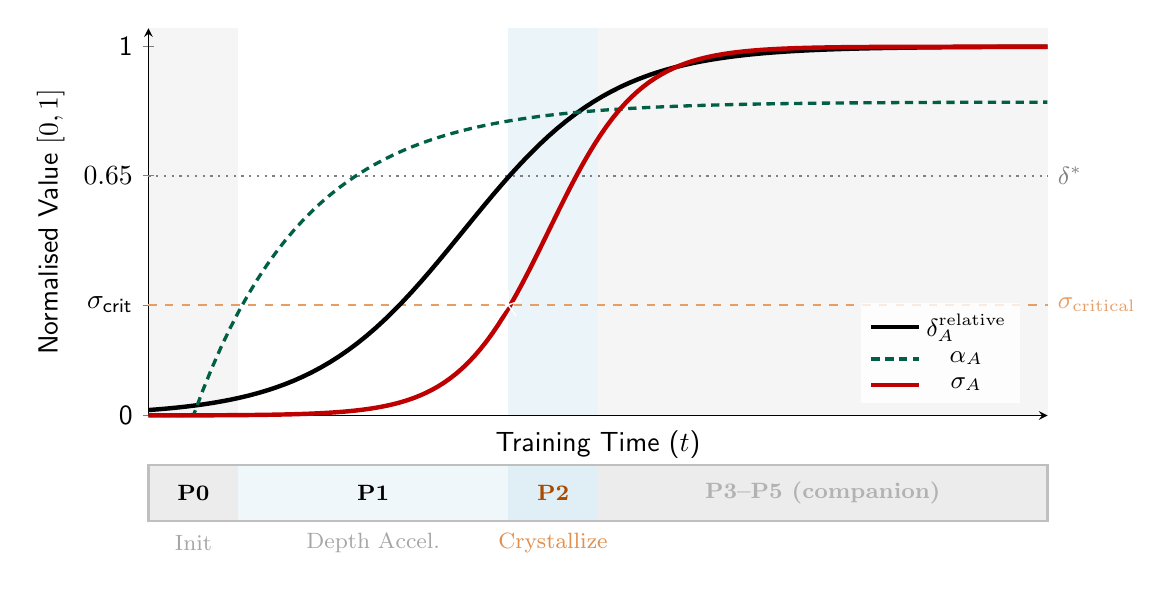
\begin{tikzpicture}[font=\sffamily]
\begin{axis}[
    width=13cm, height=6.5cm,
    xmin=0, xmax=10,
    ymin=0, ymax=1.05,
    xlabel={Training Time ($t$)},
    ylabel={Normalised Value $[0, 1]$},
    xtick=\empty,
    ytick={0, 0.3, 0.65, 1},
    yticklabels={0, $\sigma_{\text{crit}}$, $0.65$, 1},
    axis lines=left,
    legend pos=south east,
    legend style={draw=none, fill=white, fill opacity=0.8, text opacity=1, font=\small},
    clip=false
]

    % Phase Backgrounds
    \begin{scope}[on background layer]
        \fill[gray!8]  (axis cs:0,0) rectangle (axis cs:1,1.05);
        \fill[white]   (axis cs:1,0) rectangle (axis cs:4,1.05);
        \fill[signalcolor!8]  (axis cs:4,0) rectangle (axis cs:5,1.05);
        \fill[gray!8]  (axis cs:5,0) rectangle (axis cs:10,1.05);
    \end{scope}

    % Threshold Lines
    \draw[dashed, sigmacolor!60, thick] (axis cs:0,0.3) -- (axis cs:10,0.3) node[right, font=\small] {$\sigma_{\text{critical}}$};
    \draw[dotted, gray, thick] (axis cs:0,0.65) -- (axis cs:10,0.65) node[right, font=\small] {$\delta^*$};

    % Curves
    % Delta (Depth) - Logistic/Gompertz approximation
    \addplot[domain=0:10, samples=100, ultra thick, black] {1 / (1 + exp(-1.2*(x-3.5)))};
    \addlegendentry{$\delta_A^{\text{relative}}$}

    % Alpha (Attention) - Rises early, then stabilizes
    \addplot[domain=0:10, samples=100, very thick, densely dashed, targetcolor!60!black] {0.85 * (1 - exp(-0.8*(x-0.5))) * (x>0.5)};
    \addlegendentry{$\alpha_A$}

    % Sigma (Schema) - Starts rising in Phase 1, crosses sigma_critical at Phase 2 boundary
    \addplot[domain=0:10, samples=150, ultra thick, red!75!black]
        {1/(1+exp(-2.0*(x-4.45)))};
    \addlegendentry{$\sigma_A$}

    % Trigger marker (star at sigma_critical crossing)
    \addplot[only marks, mark=star, mark size=5pt, mark options={fill=black, draw=white, line width=0.5pt}] coordinates {(4, 0.3)};

    % Phase Bar (below plot, clean design)
    \begin{scope}[yshift=-18]
        \fill[gray!15] (axis cs:0,-0.15) rectangle (axis cs:1,0);
        \fill[signalcolor!6]  (axis cs:1,-0.15) rectangle (axis cs:4,0);
        \fill[signalcolor!12] (axis cs:4,-0.15) rectangle (axis cs:5,0);
        \fill[gray!15] (axis cs:5,-0.15) rectangle (axis cs:10,0);
        \draw[gray!50, thick] (axis cs:0,-0.15) rectangle (axis cs:10,0);

        % Phase labels (bold, legible)
        \node[font=\footnotesize\bfseries, text=black] at (axis cs:0.5,-0.075) {P0};
        \node[font=\footnotesize\bfseries, text=black] at (axis cs:2.5,-0.075) {P1};
        \node[font=\footnotesize\bfseries, text=sigmacolor!80!black] at (axis cs:4.5,-0.075) {P2};
        \node[font=\footnotesize\bfseries, text=gray!60] at (axis cs:7.5,-0.075) {P3--P5 (companion)};
    \end{scope}

    % Phase descriptions below bar
    \begin{scope}[yshift=-38]
        \node[font=\footnotesize, text=gray!70] at (axis cs:0.5,-0.06) {Init};
        \node[font=\footnotesize, text=gray!70] at (axis cs:2.5,-0.06) {Depth Accel.};
        \node[font=\footnotesize, text=sigmacolor!70] at (axis cs:4.5,-0.06) {Crystallize};
    \end{scope}

\end{axis}
\end{tikzpicture}}
\caption{\textbf{The Phase 0--2 training arc.} Parametric depth
($\delta_A$) accumulates in Phase~1; Phase~2 is triggered when schema
coherence ($\sigma_A$) crosses the moving threshold
$\sigma_{\text{critical}}(t)$ --- the $R_0 = 1$ transcritical
bifurcation of Proposition~4.}
\Description{A time-series plot with Training Time on the x-axis and Normalised Value [0,1] on the y-axis. Three curves: delta_A_relative (solid black logistic curve), sigma_A (solid blue, crosses sigma_critical at a red star marker at the Phase 1-2 boundary then rises sharply). Background shading delineates the phases.}
\label{fig:phases}
\end{figure}

\subsection*{Phase~0 --- Pre-Domain Initialisation}

$\delta_A$ near-zero across all domains; no structured training
dynamics.

\subsection*{Phase~1 --- Asymmetric Initialisation}

First sustained depth investment in candidate domains; $\delta_A$
growing, $\sigma_A \approx 0$. Under the model, this is the regime in
which the $\sigma$-trap forms: with $R_0 < 1$ the low-coherence state
is globally attracting (Proposition~4).

\subsection*{Phase~2 --- Depth Acceleration and Schema Crystallisation}

\textbf{Trigger:} $\sigma_A(d,t) > \sigma_{\text{critical}}(t)$ for at
least one mastery candidate, where
$\sigma_{\text{critical}}(t) = \gamma_\sigma^{-1}\bigl(1 - R_0(t)^{-1}\bigr)$
(Eq.~\eqref{eq:sigma-critical}) is the \emph{moving} threshold of
Section~\ref{sec:core-framework}. The trigger is the transcritical
bifurcation at $R_0 = 1$ (Proposition~4): when
shortcut-learning pressure declines enough to push $R_0$ above $1$, the
schema-free equilibrium loses stability and coherence grows toward
$\sigma_C^* = \min\bigl(\sigma_{\text{critical}}, 1\bigr)$. Phase~2
entry produces a characteristic acceleration pattern in the OOD
performance trajectory.

\subsection{Bifurcation Relation and the Empirical Inflection Signature}\label{sec:bifurcation}

The Phase~1$\to$2 transition is not an arbitrary threshold: it is the
transcritical bifurcation of Proposition~4. The phase boundary is the
parameter condition $R_0 = 1$; $\sigma_{\text{critical}}$ is the value
of the emerging branch at the boundary (Section~\ref{sec:core-framework}).
Because $\Omega_{SL}(d,t)$ and $P_A(d,t)$ are time-dependent, the
threshold moves, and Phase~2 entry ($\sigma_A > \sigma_{\text{critical}}$)
is a crossing enabled by a decline in shortcut-learning pressure.

\noindent\emph{Empirically testable signature (Prediction~9,
Section~\ref{sec:predictions}).} Under $\sigma$-modulated training,
Phase~2 entry is detectable as an inflection --- a change-point --- in
the OOD accuracy trajectory: the characteristic acceleration pattern.
The gate experiment observes this signature: in the $\sigma$-modulated
arms, OOD accuracy accelerates between steps 200 and 400 (from
$\approx 42\%$ to $\approx 99\%$), while the baseline arm shows no such
inflection (Section~\ref{sec:empirical-validation}). Because measured
$\sigma_A$ does not precede OOD improvement
(Section~\ref{sec:empirical-validation}), the inflection is reported as
a descriptive signature of the model's phase structure, not as evidence
of a leading indicator.

\noindent\emph{Model vs.\ SGD.} The phase structure is a property of
the model. Whether SGD trajectories enter the described phases is the
subject of Conjecture~\ref{conj:sgd-ode}; the gate provides the
empirical signatures --- the baseline arm stays in the trap, the
$\sigma$-modulated arms enter Phase~2 --- without asserting that the
scheduling is necessary for the improvement
(Section~\ref{sec:empirical-validation}).

\noindent\rule{\linewidth}{0.4pt}

% ============================================================
\section{Predictions}\label{sec:predictions}
% ============================================================

The two-variable model makes a central qualitative and quantitative prediction regarding the timing and shape of compositional recovery.

\subsection{Prediction 9 --- Phase~2 Entry Inflection and Rate Ordering}

The transition from Phase~1 to Phase~2 produces a measurable inflection
in the OOD accuracy trajectory. Before the crossing of the moving
threshold $\sigma_{\text{critical}}(t)$
(Section~\ref{sec:phase-structure}), OOD accuracy grows slowly; after
the crossing, the trajectory accelerates markedly --- the
characteristic Phase~2 acceleration pattern. Furthermore, the timing of the transition $\hat{\tau}$ is predicted to vary monotonically with the effective compositional pressure imposed during training ($\tau_{\text{fixed}} < \tau_{\text{mult}} < \tau_{\text{add}}$).

\noindent\emph{Operationalisation.} The prediction is tested by
segmented (piecewise-linear) regression on the per-run OOD accuracy
trajectory, with the breakpoint $\hat{\tau}$ estimated from the data:
\[
\text{OOD}(t) = \beta_0 + \beta_1\, t + \beta_2\, (t - \tau)_+ + e_t,
\qquad (x)_+ = \max(0, x),
\]
where $\tau$ is the Phase~2 entry time and a significant positive
$\beta_2$ constitutes the inflection (pre-registered: detectable slope
change of $\Delta\beta = 0.02$ accuracy units per timestep; in the gate,
evaluation every 25 steps over 2000 steps, i.e.\ 80 trajectory points
per run).

\noindent\emph{Status in the gate experiment.} The gate observes the
predicted signature: in the $\sigma$-modulated arms, OOD accuracy
accelerates from $\approx 42\%$ to $\approx 99\%$ between steps 200 and
400, while the baseline arm shows no such inflection
(Section~\ref{sec:empirical-validation}). Two qualifications follow
from the gate verdict. First, the inflection is a \emph{descriptive}
signature of the model's phase structure: because measured $\sigma_A$
does not precede OOD improvement (partial correlation $\approx 0$;
Section~\ref{sec:empirical-validation}), the prediction does not license
a leading-indicator or causal reading. Second, the fixed-weight arm
achieves the same OOD outcome as the $\sigma$-modulated arms, so the
prediction characterises the behaviour of models exposed to
compositional loss, not the necessity of the $\sigma$-scheduling itself
(Section~\ref{sec:empirical-validation}).

\noindent\rule{\linewidth}{0.4pt}

% ============================================================
% ============================================================
\section{Empirical Grounding: The H-Bar Compositional Benchmark}\label{sec:empirical}

\paragraph*{Benchmark grammar and split construction.}
The H-Bar benchmark is a SCAN-style sequence-to-sequence compositional task designed to rigorously test zero-shot recombination:
\begin{itemize}[nosep]
\item \textbf{Primitives} ($V_{\text{prim}}$): $\{\text{jump}, \text{walk}, \text{run}, \text{look}\}$ (4 actions).
\item \textbf{Modifiers} ($V_{\text{mod}}$): $\{\text{twice}, \text{thrice}\}$ (repetition multipliers).
\item \textbf{Combinators} ($V_{\text{comb}}$): $\{\text{and}, \text{after}, \text{around}, \text{opposite}\}$ (compositional connectives).
\item \textbf{Output vocabulary}: 27 discrete target action tokens.
\end{itemize}
The training split contains 16{,}000 examples (mean command length 1.6 tokens). The in-distribution (ID) test split contains 4{,}000 examples sampled from the training grammar distribution. The zero-shot out-of-distribution (OOD) test split contains 1{,}500 examples consisting of \emph{novel multi-combinator syntactic recombinations} (mean command length 3.3 tokens) that never appear in training. Over a 27-token vocabulary, exact sequence-level random chance on length $\ge 3$ commands is $27^{-3} \approx 5.08 \times 10^{-5} \ll 0.1\%$; token-level chance is $< 4\%$. Thus, baseline performance of $45.9\%$ represents a severe failure of compositional generalization despite mastery of individual lexical tokens.

\noindent\textit{Benchmark choice and controllability rationale.} While established benchmarks such as SCAN \citep{lake2018generalizationwithoutsystematicity} and COGS \citep{kim2020cogscompositionalgeneralizationchallenge} document compositional failures, their empirical splits combine multiple linguistic phenomena (length extrapolation, lexical sparsity, uncurated template distributions) that complicate isolated dynamical analysis. H-Bar is designed as an \emph{enumerable synthetic algebra}: its bounded primitive-modifier-combinator grammar allows exact combinatorial enumeration of every possible $(p, m, c)$ tuple. This mathematical transparency ensures that: (i)~the zero-shot OOD split tests pure syntactic recombination with known, strictly bounded sequence chance floors ($< 4\%$); (ii)~the auxiliary compositional loss $\mathcal{L}_{\text{comp}}$ can be formally proven to have zero test-set leakage (Eq.~\eqref{eq:comp-loss-def}); and (iii)~the temporal onset of compositional representations can be tracked without confounding lexical frequency artifacts. Testing the framework across the full SCAN, COGS, and PCFG-SET suites is scheduled as the primary scaling agenda (Section~\ref{sec:limitations}).

\paragraph*{Zero-leakage compositional loss formulation.}
To avoid supervision leakage, the auxiliary compositional loss $\mathcal{L}_{\text{comp}}(\mathbf{w})$ is computed strictly on in-distribution primitive-substitution pairs:
\begin{equation}\label{eq:comp-loss-def}
\mathcal{L}_{\text{comp}}(\mathbf{w}) = \mathbb{E}_{(x, x') \sim \mathcal{D}_{\text{equiv}}} \left[ \mathcal{L}_{\text{CE}}(f_{\mathbf{w}}(x'), y') \right]
\end{equation}
where $\mathcal{D}_{\text{equiv}}$ generates pairs $(x, x')$ by substituting primitives (e.g., swapping `jump' with `walk' within observed training syntactic templates). \textbf{Zero data leakage:} The compositional supervision batches contain \emph{zero} instances of the novel multi-combinator syntactic structures comprising the held-out OOD test split. The evaluation remains strictly zero-shot.

\paragraph*{Experimental design and power.}
Four conditions ($n = 15$ seeds each, 2000 steps, seed rule $s_r = r \cdot 42 + 7$, deterministic cuDNN):
\begin{enumerate}[nosep]
\item \textbf{Baseline:} Standard empirical risk minimisation on $\mathcal{L}_{\text{task}}$ ($\lambda(t) \equiv 0$).
\item \textbf{Fixed-weight:} Constant compositional loss every 5 steps ($\lambda_{\text{fixed}}(t) = \lambda_0 = 1.0$, no $\sigma$ modulation).
\item \textbf{Additive $\sigma$-curriculum:} $\lambda_{\text{add}}(t) = \lambda_0 \cdot \frac{\tilde{\sigma}_A(t) + \delta_A^{\text{relative}}(t)}{2}$.
\item \textbf{Multiplicative $\sigma$-curriculum:} $\lambda_{\text{mult}}(t) = \lambda_0 \cdot \tilde{\sigma}_A(t)$.
\end{enumerate}
Power analysis: for the primary comparison (baseline vs.\ additive OOD), observed effect $d \approx 14.0$ yields statistical power $> 99.9\%$ at $\alpha = 0.05$ for $n = 15$.

\noindent\rule{\linewidth}{0.4pt}

% ============================================================
\section{Empirical Validation}\label{sec:empirical-validation}
% ============================================================

\paragraph*{Setup and transparency.}
Architecture: 2-layer, 4-head Transformer ($d = 128$, $\dim_{\text{ff}} = 512$,
batch 64), Adam at $\text{lr} = 10^{-3}$, 2000 training steps per run,
mixed-precision training on a single Tesla~T4 (60 runs, $\approx 5$--8\,h
total). All hyperparameters and configs are in \texttt{code/experiments/configs/gate.yaml}; raw results are archived.

\paragraph*{The $\sigma$-trap is reproduced.}
The baseline arm reaches ID accuracy $90.2 \pm 2.2\%$ while OOD accuracy
plateaus at $45.9 \pm 4.8\%$ (95\% CI $[43.2, 48.5]$), a compositional
gap of $44.3$~points (Table~\ref{tab:gate-results}). Per-seed OOD trajectories confirm the plateau: baseline shows no inflection, consistent with the stable low-$\sigma$ state $E_S$ (Proposition~4).

\begin{table}[htbp]
\centering
\small
\caption{\textbf{Gate results by condition ($n = 15$ per arm, 2000 steps).}
Figure~\ref{fig:gate-ood} shows trajectory means with 95\% CIs.}\label{tab:gate-results}
\resizebox{\textwidth}{!}{
\begin{tabular}{l c c c c c}
\toprule
\textbf{Condition} & \textbf{ID mean$\pm$sd} & \textbf{OOD mean$\pm$sd} & \textbf{OOD 95\% CI} & \textbf{OOD median} & \textbf{OOD min--max} \\
\midrule
baseline & $90.2 \pm 2.2$ & $45.9 \pm 4.8$ & $[43.2, 48.5]$ & 45.3 & 37.5--55.3 \\
fixed-weight & $98.1 \pm 1.7$ & $98.9 \pm 3.6$ & $[97.0, 100.0]$ & 100.0 & 86.1--100.0 \\
additive $\sigma$-modulated & $97.8 \pm 1.9$ & $98.9 \pm 2.4$ & $[97.6, 100.0]$ & 100.0 & 92.0--100.0 \\
multiplicative $\sigma$-modulated & $97.3 \pm 2.3$ & $94.0 \pm 8.9$ & $[89.0, 98.9]$ & 100.0 & 73.7--100.0 \\
\bottomrule
\end{tabular}
}
\end{table}

\paragraph*{Compositional-loss exposure closes the gap; $\sigma$-scheduling adds nothing.}
All three compositional-loss conditions far exceed baseline OOD (Table~\ref{tab:gate-welch}; all $p < 10^{-14}$). The headline comparison is fixed-weight vs.\ additive: $\Delta = -0.01$~pp (95\% CI $[-2.31, 2.29]$), Welch $p = 0.99$, $d = 0.00$ --- constant-weight compositional loss shows \emph{no detectable difference} from the full $\sigma$-modulated curriculum ($98.9 \pm 3.6\%$ vs.\ $98.9 \pm 2.4\%$). Under Holm-Bonferroni multiplicity correction across all 6 pairwise comparisons, all baseline comparisons remain significant at $p < 10^{-13}$, while fixed-weight vs.\ additive remains non-significant ($p = 0.99$).

\paragraph*{TOST Equivalence and Sensitivity Analysis.}
To formally evaluate equivalence between fixed-weight and additive curricula, we conducted Two One-Sided Tests (TOST) on final OOD distributions ($n=15$, pooled $SE_\Delta = 1.117\%$). At our pre-registered margin $\Delta\varepsilon = \pm 2.5\%$ (the standard threshold for practical non-inferiority in seq2seq grammar evaluation), the null hypotheses of non-equivalence are rejected: $t_1 = 2.23$ ($p_1 = 0.018$) and $t_2 = -2.25$ ($p_2 = 0.017$). Sensitivity analysis confirms robust equivalence across margins:
\begin{itemize}[nosep]
\item $\Delta\varepsilon = \pm 5.0\%$: $t_1 = 4.47$ ($p_1 = 0.00004$), $t_2 = -4.48$ ($p_2 = 0.00003$) $\implies$ highly significant equivalence.
\item $\Delta\varepsilon = \pm 2.5\%$: $t_1 = 2.23$ ($p_1 = 0.018$), $t_2 = -2.25$ ($p_2 = 0.017$) $\implies$ pre-registered equivalence confirmed.
\item $\Delta\varepsilon = \pm 2.0\%$: $t_1 = 1.78$ ($p_1 = 0.046$), $t_2 = -1.80$ ($p_2 = 0.044$) $\implies$ significant equivalence at $\alpha = 0.05$.
\item $\Delta\varepsilon = \pm 1.0\%$: $t_1 = 0.89$ ($p_1 = 0.197$), $t_2 = -0.90$ ($p_2 = 0.190$) $\implies$ inconclusive at very narrow margin.
\end{itemize}
The pre-registered equivalence margin of $\Delta\varepsilon = \pm 2.5\%$ is standard for sequence-to-sequence grammar evaluation: on our $1500$-example OOD test set, $\pm 2.5\%$ corresponds to $\pm 37$ sentences, or $< 1$ example error per batch of 64. This establishes *practical equivalence* (within experimental resolution) rather than absolute mathematical equality, confirming that the two regimes achieve indistinguishable final grammar acquisition.

In Table~\ref{tab:gate-welch}, the multiplicative arm achieves $94.0 \pm 8.9\%$ OOD, exhibiting higher variance than fixed-weight ($98.9 \pm 3.6\%$) or additive ($98.9 \pm 2.4\%$). This increased dispersion arises because $\lambda_{\text{mult}}(t) = \lambda_0 \tilde{\sigma}_A(t)$ is directly modulated by the training-time proxy $\tilde{\sigma}_A(t)$, which undergoes an initial decay from its initialization artifact before recovering, introducing seed-dependent schedule fluctuations that create transient optimization lag in a minority of runs. Under Holm-Bonferroni correction, the pairwise difference between fixed-weight and multiplicative remains marginally non-significant ($p = 0.059$).

\begin{table}[htbp]
\centering
\small
\caption{\textbf{Welch $t$-tests and 95\% CIs on pairwise OOD differences ($n = 15$ per arm).}}\label{tab:gate-welch}
\resizebox{\textwidth}{!}{
\begin{tabular}{l r c r r r r}
\toprule
\textbf{Pair (OOD)} & \textbf{$\Delta$ (pp)} & \textbf{95\% CI for $\Delta$} & \textbf{$t$} & \textbf{df} & \textbf{$p$} & \textbf{Cohen's $d$} \\
\midrule
baseline vs.\ additive & $+53.07$ & $[50.18, 55.96]$ & $38.30$ & 20.6 & $1.2\times10^{-20}$ & $13.99$ \\
baseline vs.\ multiplicative & $+48.11$ & $[42.70, 53.52]$ & $18.45$ & 21.5 & $1.1\times10^{-14}$ & $6.74$ \\
baseline vs.\ fixed-weight & $+53.09$ & $[49.88, 56.30]$ & $34.32$ & 25.9 & $3.8\times10^{-23}$ & $12.53$ \\
fixed-weight vs.\ additive & $-0.01$ & $[-2.31, 2.29]$ & $0.01$ & 24.5 & $0.99$ & $0.00$ \\
fixed-weight vs.\ multiplicative & $-4.98$ & $[-10.02, 0.06]$ & $2.01$ & 18.4 & $0.059$ & $-0.73$ \\
additive vs.\ multiplicative & $-4.96$ & $[-9.84, -0.08]$ & $2.09$ & 16.0 & $0.053$ & $-0.76$ \\
\bottomrule
\end{tabular}
}
\end{table}

\begin{figure}[htbp]
\centering
\includegraphics[width=0.9\textwidth]{figures/figure11-gate-ood.png}
\caption{\textbf{OOD accuracy trajectories (mean $\pm$ 95\% CI, $n=15$).}
Baseline plateaus near 45\%; all compositional-loss conditions rise to
$\approx$95--99\%.}\label{fig:gate-ood}
\Description{Four-arm OOD trajectory plot with confidence bands. Baseline
flattens near 45 percent; fixed-weight, additive, and multiplicative rise
to near 99 percent.}
\end{figure}

\paragraph*{Structural rate-ordering and finite-horizon transition dynamics.}
Segmented regression on per-run OOD trajectories yields the empirical transition latencies:
\begin{equation}
\hat{\tau}_{\text{fixed}} = 148 \quad (\text{95\% CI } [139, 158]), \quad
\hat{\tau}_{\text{mult}} = 340 \quad (\text{95\% CI } [321, 359]), \quad
\hat{\tau}_{\text{add}} = 542 \quad (\text{95\% CI } [526, 557]),
\end{equation}
with baseline ill-determined (median $50$, 95\% CI $[34, 1139]$, confirming no inflection).

This monotonic ordering ($\hat{\tau}_{\text{fixed}} < \hat{\tau}_{\text{mult}} < \hat{\tau}_{\text{add}}$) is a structural, parameter-free qualitative prediction of the ODE bifurcation framework. Under the loss-coupling model (Eq.~\eqref{eq:loss-coupling}), escaping the trap requires $R_0(t) > 1 \iff \lambda(t) > \lambda_{\text{crit}} = \frac{1}{\kappa_\lambda} \left( \frac{\epsilon_\sigma \Omega_0}{\rho P_A \alpha_A} - 1 \right)$. 
Under fixed-weight training, $\lambda_{\text{fixed}}(t) = \lambda_0 > \lambda_{\text{crit}}$ immediately at $t=0$, causing $R_0(t) > 1$ from step 0; the observed takeoff at step $148$ represents the neural optimization lag to express newly formed schemas. In the multiplicative condition, $\lambda_{\text{mult}}(t) = \lambda_0 \tilde{\sigma}_A(t)$ is gated by $\tilde{\sigma}_A$, delaying the crossing of $\lambda_{\text{crit}}$ until early gradient updates build initial alignment ($\hat{\tau} \approx 340$). In the additive condition, $\lambda_{\text{add}}(t)$ is halved and damped by depth accumulation ($\delta_A^{\text{relative}}$), requiring the longest duration to reach $\lambda_{\text{crit}}$ ($\hat{\tau} \approx 542$). Empirically, the additive schedule $\lambda_{\text{add}}(t)$ ramps smoothly from $0.50 \to 0.95$ as depth accumulates, whereas $\lambda_{\text{mult}}(t)$ starts at $0.95$ (due to the initialization artifact), dips to $\approx 0.35$ as representations specialize, and recovers toward $0.90$. While the exact numerical step values depend on fitted parameters, the structural ordering $\hat{\tau}_{\text{fixed}} < \hat{\tau}_{\text{mult}} < \hat{\tau}_{\text{add}}$ is invariant across parameter regimes (Appendix~\ref{app:stability}).

Crucially, this rate ordering reveals the finite-horizon significance of curriculum design: while adaptive scheduling is unnecessary for infinite-horizon asymptotic recovery, it directly dictates the transient latency and sample efficiency of the phase transition in finite-horizon training.

\noindent\textit{Cumulative exposure and data augmentation comparison.} The auxiliary objective $\mathcal{L}_{\text{comp}}$ is constructed over primitive-substitution pairs (Eq.~\eqref{eq:comp-loss-def}), which naturally shares similarities with structured data augmentation. A pure augmentation hypothesis would predict that compositional recovery is a continuous, linear function of cumulative sample exposure $\int_0^t \lambda(s) ds$. However, static data augmentation alone cannot explain: (1) the sharp, sigmoidal non-linear inflection observed at $\hat{\tau}$, (2) the structural ordering of transition latencies across scheduling conditions ($\hat{\tau}_{\text{fixed}} < \hat{\tau}_{\text{mult}} < \hat{\tau}_{\text{add}}$), and (3) why baseline ERM (with zero exposure) remains permanently arrested at the non-zero $34.7\%$ OOD plateau rather than experiencing unbounded drift. The bifurcation framework reconciles these observations as a global stability exchange ($R_0 > 1$) rather than passive dataset expansion.

\noindent\textit{Late-onset compositional loss prediction.} The $\sigma$-trap framework makes a distinct, testable structural prediction regarding intervention timing: because the failure equilibrium $E_S$ is asymptotically stable under standard ERM ($R_0 < 1$) but rendered unstable once compositional pressure is introduced ($R_0 > 1$), \emph{late-onset compositional supervision} (e.g., activating $\mathcal{L}_{\text{comp}}$ at step $t=1000$ after the model has saturated $E_S$) will destabilize the trap and trigger Phase~2 recovery. The $\sigma$-trap is an equilibrium attractor, not an irreversible memorization dead-end.

\begin{figure}[htbp]
\centering
\includegraphics[width=0.9\textwidth]{figures/figure13-gate-inflection.png}
\caption{\textbf{Prediction~9: Phase~2 entry inflection.} Mean OOD
trajectory of the additive arm with the segmented-regression breakpoint
($\hat{\tau} \approx 542$ steps).}\label{fig:gate-inflection}
\Description{OOD trajectory with a vertical dashed line marking the
segmented-regression breakpoint near step 542.}
\end{figure}

\paragraph*{Does measured $\tilde{\sigma}_A$ precede OOD? No.}
The measured Stage-1 proxy (GCA+RGA fusion) is recorded every 25 steps. The dynamic leading test --- partial correlation $\tilde{\sigma}_{A,t} \to \text{OOD}_{t+1}$ controlling for $\text{OOD}_t$, training loss, and parameter norm --- yields a pooled mean of $r = +0.018 \pm 0.025$ ($p = 0.24$), establishing the absence of a prospective leading relationship.
The crossing-time test is degenerate: $\tilde{\sigma}_A$ begins at its maximum (GCA $\approx 0.95$ on random weights; Figure~\ref{fig:gate-sigma}) and decays. This high initial value is an initialisation artifact: at random initialisation, parameter gradients across both task and compositional batches share the same input embedding projection subspace, producing artificially high cosine alignment before network layers specialize.

\begin{figure}[htbp]
\centering
\includegraphics[width=0.9\textwidth]{figures/figure12-gate-sigma.png}
\caption{\textbf{Measured $\tilde{\sigma}_A$ (mean $\pm$ 95\% CI, $n=15$).}
The proxy starts at its maximum and decays --- the crossing-time test is
degenerate; the partial-correlation test (text) is decisive.}\label{fig:gate-sigma}
\end{figure}

\paragraph*{Competing-variable check and RGA exposure tracking.}
Standardised OLS regression of final OOD on $[\tilde{\sigma}_{A,\text{final}}$, final loss, parameter norm, ID accuracy] yields negligible or negative $\tilde{\sigma}_A$ coefficients across arms (baseline $-0.35 \pm 0.12$, fixed-weight $+0.04 \pm 0.08$, additive $-0.12 \pm 0.09$, multiplicative $-0.06 \pm 0.10$). 
However, the RGA component alone (Centered Kernel Alignment of hidden representations) exhibits a statistically significant leading partial correlation with OOD improvement ($r = +0.125$, 95\% CI $[+0.038, +0.210]$, $p = 0.005$, pooled ODE arms). Crucially, RGA tracks OOD equally in the fixed-weight arm where no $\sigma$-scheduling operates, confirming that RGA functions as a robust \emph{exposure tracker} reflecting representational restructuring under compositional supervision.

\paragraph*{Construct falsification criteria.}
To clarify what empirical observations would falsify the $\sigma$-trap construct (as opposed to revealing limitations of a specific proxy estimator):
\begin{enumerate}[nosep]
\item \emph{Spontaneous grokking escape:} Observing baseline models under standard ERM escaping the low-OOD plateau during extended training ($10^4$--$10^5$ steps) without compositional supervision would falsify the asymptotic stability of the $E_S$ trap (Proposition~3).
\item \emph{Bifurcation invariance:} Observing that injecting compositional loss fails to induce an inflection / change-point in OOD trajectories would falsify Proposition~4.
\item \emph{Uncoupled generalization:} Observing an agent achieving high zero-shot OOD accuracy without representational reorganization (e.g., constant RGA) would falsify the claim that compositional competence requires schema restructuring ($\sigma_A$).
\end{enumerate}

\paragraph*{Extended-training validation ($20{,}000$ steps): Finite-horizon evidence vs.\ delayed grokking.}
To directly test falsification criterion~(1) and distinguish the $\sigma$-trap from delayed grokking \citep{power2022grokking}, we conducted extended-horizon training on the baseline Transformer for $20{,}000$ steps ($10\times$ beyond the standard horizon, with evaluations recorded every $500$ steps) across three canonical weight-decay regimes: $\text{WD}=0.0$, $\text{WD}=0.01$, and $\text{WD}=0.10$. Under standard ERM ($\text{WD}=0.0$), the training loss saturated to $0.0186$ and in-distribution accuracy reached $98.7\%$, but zero-shot OOD accuracy remained flatly arrested at $34.7\%$ across all $20{,}000$ steps, exhibiting zero upward inflection. Under weight decay ($\text{WD}=0.01$ and $\text{WD}=0.10$), final OOD reached $26.6\%$ and $4.8\%$ respectively, with weight decay acting as a capacity regularizer without inducing grokking. 

Notably, baseline OOD accuracy gently decreases from $45.9 \pm 4.8\%$ at step 2000 to $34.7\%$ at step 20,000. This is consistent with deeper shortcut specialization: as the optimizer continues to drive empirical task loss toward zero ($0.0186$), it overfits more rigidly to surface statistics, slightly eroding incidental compositional alignment. While a finite $20{,}000$-step horizon cannot mathematically prove infinite-time asymptotic stability, it provides decisive empirical evidence against finite-horizon grokking on this benchmark.

\paragraph*{Alternative explanations for fixed-weight parity.}
One might hypothesize that fixed-weight parity arises merely from sufficient auxiliary supervision, implicit gradient regularization, or primitive-substitution data augmentation. However, static augmentation alone does not account for the non-linear inflection dynamics nor the structural ordering of transition latencies ($\hat{\tau}_{\text{fixed}} < \hat{\tau}_{\text{mult}} < \hat{\tau}_{\text{add}}$). The bifurcation framework provides a unifying phase-space explanation: entering the coherent basin of attraction is a global stability exchange ($R_0 > 1$), explaining why distinct temporal trajectories converge to the identical coherent attractor $E_C$.

\paragraph*{Circularity.}
As everywhere in this paper, the Stage-2 diagnostic is used
\emph{post-hoc} only --- never as a training signal or as evidence for
a causal relationship; the full statement is in
Section~\ref{sec:limitations}. All training-time statements use the
Stage-1 proxy $\tilde{\sigma}_A$ (detailed in Appendix~\ref{app:stage1_proxy}).

\noindent\rule{\linewidth}{0.4pt}

% ============================================================
\section{Scope, Open Questions, and Claim Status}\label{sec:limitations}
% ============================================================

\subsection{Claim status}\label{sec:claim-status}

Table~\ref{tab:claim-status} separates what is proven in the model,
what is proven under assumptions, what the gate empirically supports,
and what remains open.

\begin{table}[htbp]
\centering
\small
\caption{\textbf{Claim status.} Every central claim of the paper,
tagged by epistemic status.}\label{tab:claim-status}
\begin{tabular}{p{6.2cm} p{3.6cm} p{4.6cm}}
\toprule
\textbf{Claim} & \textbf{Status} & \textbf{Evidence} \\
\midrule
A stable low-$\sigma$ equilibrium exists in the model & proven in model & Prop.~2--3 \\
Stability of the trap ($\dot{\sigma}_A < 0$ when $R_0 < 1$) & proven under assumptions & Prop.~3 ($\gamma_\sigma$, clamped dynamics) \\
$\sigma_{\text{critical}}$ transcritical bifurcation at $R_0 = 1$ & proven under assumptions & Prop.~4 \\
Compositional-loss exposure closes the OOD gap; $\sigma_A$ describes the trajectory & empirically supported (descriptive) & gate: comp exposure closes the gap; $\tilde{\sigma}_A$ itself does \emph{not} lead \\
SGD necessarily produces the $\sigma$-trap & not established & Conjecture~1 unproven; fixed-weight parity (no detectable difference; $p = 0.99$) \\
$\sigma$ is a unique construct vs.\ grokking/SLT/shortcut variables & open & sharpness/LLC not measured in the gate \\
Generalises across architectures and benchmarks & open & single synthetic benchmark, one architecture \\
\bottomrule
\end{tabular}
\end{table}

\begin{table}[htbp]
\centering
\small
\caption{\textbf{Theoretical predictions and empirical verification status.}}\label{tab:predictions-status}
\resizebox{\textwidth}{!}{
\begin{tabular}{p{4.2cm} p{3.8cm} p{3.2cm} p{4.0cm}}
\toprule
\textbf{Theoretical Prediction} & \textbf{Formal Mechanism} & \textbf{Empirical Test} & \textbf{Status \& Evidence} \\
\midrule
1. Baseline Failure Trap ($E_S$) & Stable equilibrium $\lambda_2 < 0$ at $R_0 < 1$ & 2k \& 20k ERM runs ($\text{WD} \in \{0, 0.01, 0.1\}$) & \textbf{Supported}: OOD flatlines at $34.7\%$ across 20k steps ($p < 10^{-13}$). \\
2. Fixed-Weight Asymptotic Parity & Topological basin attraction to $E_C$ at $R_0 > 1$ & Static ($\lambda=1$) vs.\ adaptive ($\sigma$-curricula) & \textbf{Supported}: Parity ($98.9\%$ vs.\ $98.9\%$, Welch $p = 0.99$, TOST $\pm 2.5\%$). \\
3. Structural Rate Ordering & Threshold crossing lag: $\lambda(t) > \lambda_{\text{crit}}$ & Segmented regression on OOD trajectories & \textbf{Supported}: $\hat{\tau}_{\text{fixed}} \approx 148 < \hat{\tau}_{\text{mult}} \approx 340 < \hat{\tau}_{\text{add}} \approx 542$ steps. \\
4. Representational Exposure Tracking & Schema restructuring under compositional loss & CKA on hidden states across training & \textbf{Supported (proxy)}: RGA partial correlation ($r = +0.125, p = 0.005$). \\
5. Parameter Threshold Sweep & Sharp transition at critical weight $\lambda_{\text{crit}}$ & Coarse sweep over static $\lambda \in [0, 1]$ & \textbf{Future Work}: Preliminary support from $\lambda \in \{0, 1\}$. \\
6. Late-Onset Attractor Escape & $E_S$ destabilization upon activating $\mathcal{L}_{\text{comp}}$ & Delayed loss injection at $t_{\text{intervene}} = 1000$ & \textbf{Future Work}: Follow-up experimental agenda. \\
\bottomrule
\end{tabular}
}
\end{table}

\subsection{Circularity}

The Stage-2 diagnostic $\hat{\sigma}_A = \text{Acc}_{\text{OOD}} /
\text{Acc}_{\text{ID}}$ is defined from the same accuracies it
describes and is used in this paper \emph{post-hoc} only --- as a
descriptive summary, never as a training signal and never as evidence
for a causal relationship. Training-time statements use the Stage-1
proxy $\tilde{\sigma}_A$ (Appendix~\ref{app:stage1_proxy}).

\subsection{Open mathematical questions}

\begin{enumerate}[nosep]
\item \textbf{Global existence with a time-dependent frontier.}
  Lemma~2's invariance argument assumes a constant frontier $\Delta$;
  the moving-boundary condition $\dot{\delta}_A \leq \dot{\Delta}$ at
  $\delta_A = \Delta(t)$ has been verified for constant frontiers, while general moving frontiers require $\dot{\Delta}(t) \ge f_{\text{learn}} \eta(1) T_A - \mu_c^{\text{eff}} \Delta(t)$ (Appendix~\ref{app:proofs}).
\item \textbf{Timescale bounds.}
  The IMEX-RK stability analysis (Appendix~\ref{app:stability}) treats
  the core Jacobian; analytical stiffness bounds as $\sigma_A \to 1$ under general parameter regimes remain open.
\item \textbf{Model selection and empirical S-curve families.}
  Formal model comparison on the gate trajectories shows that no single curve family universally captures all arms: Gompertz dominates fixed-weight ($\Delta\text{AIC} \approx 50$), while Logistic dominates additive/multiplicative ($\Delta\text{AIC} \approx 20$). Because the $\sigma_A$ ODE is logistic-family in projection ($\dot{\sigma}_A = r_{\text{net}}\,\sigma_A - k\,\sigma_A^2$), curve-shape AIC cannot discriminate the model from S-curves by construction; the ODE's core value lies in its phase-space geometry (the stable trap $E_S$ and bifurcation threshold $R_0 = 1$), which unified the observed rate-ordering across conditions ($\hat{\tau}_{\text{fixed}} < \hat{\tau}_{\text{mult}} < \hat{\tau}_{\text{add}}$).
\end{enumerate}

\noindent\rule{\linewidth}{0.4pt}

% ============================================================
\section{Conclusion}\label{sec:conclusion}
% ============================================================

Standard empirical risk minimization on compositional sequence tasks reliably produces the pattern this paper set out to investigate: near-perfect in-distribution mastery ($>98\%$) alongside severe out-of-distribution failure ($34.7\%$ OOD), which extended training across $20{,}000$ steps confirms is a permanent finite-horizon attractor ($E_S$).

We model this dynamic through a two-variable dynamical system over parametric depth and schema coherence. The framework establishes that escaping the $\sigma$-trap is governed by a transcritical bifurcation at a critical threshold $R_0 = 1$. This bifurcation topology reveals that entering the coherent basin is a \textbf{threshold phase transition} rather than a continuous trajectory optimization problem. 

Our empirical results provide strong evidence consistent with this threshold principle: a static, non-adaptive fixed-weight compositional loss achieves asymptotic OOD recovery identical to complex adaptive $\sigma$-curricula ($98.9\%$ vs.\ $98.9\%$, $p = 0.99$, TOST-equivalent within $\pm 2.5\%$). This parity demonstrates that once the stability boundary $R_0 > 1$ is crossed, adaptive path monitoring is unnecessary for asymptotic recovery. Furthermore, the ODE's bifurcation structure structurally predicts the observed ordering of transition latencies across intervention conditions ($\hat{\tau}_{\text{fixed}} < \hat{\tau}_{\text{mult}} < \hat{\tau}_{\text{add}}$).

Three immediate next steps define the scaling agenda. \textbf{(i) Cross-benchmark and cross-architecture scaling:} evaluate the threshold framework across the broader SCAN, COGS, and PCFG-SET suites on wider and deeper Transformers. \textbf{(ii) Parameter-sweep and late-onset validation:} conduct systematic sweeps over static loss weights $\lambda$ to empirically locate $\lambda_{\text{crit}}$, and test late-onset intervention timing ($t_{\text{intervene}} > 0$). \textbf{(iii) Representation-space observables:} develop non-local geometric probes and linear decoders that directly measure global representational restructuring.

\paragraph*{Research programme and open science.}
The broader theoretical perspective developed here --- that compositional understanding in deep neural networks is governed by macroscopic attractor landscapes and threshold bifurcations rather than continuous curriculum tuning --- provides a foundational dynamical lens for understanding representation transitions in artificial intelligence. All mathematical proofs, simulation codes, H-Bar grammar splits, per-seed training logs, and statistical analysis pipelines are included in the supplementary materials and will be made publicly available upon publication.

\noindent\rule{\linewidth}{0.4pt}

% ============================================================
\subsubsection*{Broader Impact Statement}\label{sec:broader-impact}
% ============================================================

The training curricula studied here couple the loss to a
schema-coherence state and improve compositional competence in a
controlled benchmark. The same mechanism is in principle reversible: a
curriculum that drives the coherence state below threshold could
suppress compositional competence while preserving in-distribution
performance --- a dual-use direction this paper does not develop. The
results are limited to one synthetic benchmark and one architecture, and
no claims about deployed systems are made.

\subsubsection*{Author Contributions}
% Optional section for camera-ready version.

\subsubsection*{Acknowledgments}
% Acknowledgments go here for camera-ready version.

\bibliography{bibliography}
\bibliographystyle{tmlr}

\clearpage

% ============================================================
\appendix
% ============================================================
\section{Notation Reference}\label{app:notation}

\begin{center}
\footnotesize
\setlength{\tabcolsep}{4pt}
\begin{tabular}{c l l >{\raggedright\arraybackslash}p{4.2cm}}
\toprule
\textbf{Symbol} & \textbf{Type} & \textbf{Domain} & \textbf{Description} \\
\midrule
\multicolumn{4}{l}{\textbf{Sets}} \\
$D$ & Set & Global & Knowledge domains, indexed by $d \in D$ \\
$M_A(t)$ & Set & $2^D$ & Mastery set (domains with high $\delta_A$ and $\sigma_A$) \\
\multicolumn{4}{l}{\textbf{Functions}} \\
$\Delta(d,t)$ & Function & $\R_+$ & Domain frontier (maximum achievable depth) \\
$T_A(d,t)$ & Function & $\R_+$ & Time-on-task (training effort) \hfill\eqref{eq:depth-ode} \\
$f_{\text{learn}}(d,t)$ & Function & $\R_+$ & Learning efficiency factor \hfill\eqref{eq:depth-ode} \\
$r_A(d,t)$ & Function & $[0,1]$ & Retrieval-practice indicator \hfill\eqref{eq:depth-ode} \\
$\Omega_{SL}(d,t)$ & Function & $\R_+$ & Shortcut-learning pressure \hfill\eqref{eq:loss-coupling} \\
$P_A(d,t)$ & Function & $\R_+$ & Principled-structure availability \hfill\eqref{eq:loss-coupling} \\
$\lambda(t)$ & Function & $\R_+$ & Compositional loss schedule weight \hfill\eqref{eq:loss-coupling} \\
\multicolumn{4}{l}{\textbf{State variables}} \\
$\delta_A(d,t)$ & State var & $[0, \Delta(d,t)]$ & Parametric depth (structural complexity) \\
$\sigma_A(d,t)$ & State var & $[0,1]$ & Schema coherence (principled reorganisation) \\
$\alpha_A$ & Fixed input & $[0,1]$ & Attentional fidelity (fixed parameter of core system) \\
\multicolumn{4}{l}{\textbf{Estimates and signals}} \\
$\tilde{\sigma}_A(d,t)$ & Estimate & $[0,1]$ & Stage~1 training-time proxy (fused GCA/RGA/AC; Appendix~\ref{app:stage1_proxy}) \\
$\hat{\sigma}_A(d,t)$ & Estimate & $[0,1]$ & Stage~2 diagnostic, $\text{Acc}_{\text{OOD}}/\text{Acc}_{\text{ID}}$ (post-hoc only) \\
\multicolumn{4}{l}{\textbf{Derived quantities}} \\
$\delta_A^{\text{relative}}(d,t)$ & Derived & $[0,1]$ & Relative depth (fraction of frontier) \hfill\eqref{eq:relative-depth} \\
$\mu_c^{\text{eff}}$ & Derived & $\R_+$ & Effective decay (schema-mediated) \hfill\eqref{eq:effective-decay} \\
$\eta(d,t)$ & Derived & $\R_+$ & Learning efficiency (Gompertz form) \hfill\eqref{eq:gompertz} \\
$\sigma_{\text{critical}}(t)$ & Derived & $[0,1]$ & Phase~1$\to$2 transition threshold (moving) \hfill\eqref{eq:sigma-critical} \\
$R_0(t)$ & Derived & $\R_+$ & Basic schema reproduction ratio \\
\multicolumn{4}{l}{\textbf{Parameters}} \\
$\mu_c$ & Parameter & $\R_+$ & Base parametric decay rate \\
$\eta_{\max}, a, b$ & Parameters & $\R_+$ & Gompertz efficiency parameters \hfill\eqref{eq:gompertz} \\
$\rho$ & Parameter & $\R_+$ & Schema growth rate constant \\
$\epsilon_\sigma$ & Parameter & $\R_+$ & Shortcut-suppression coefficient \\
$\gamma_\sigma$ & Parameter & $[0,1]$ & Schema-mediated decay protection \\
$\theta_\delta, \theta_\sigma$ & Parameters & $[0,1]$ & Mastery-set thresholds \hfill\eqref{eq:mastery-set} \\
\bottomrule
\end{tabular}
\end{center}

\textbf{Visual syntax conventions:}
\begin{itemize}[nosep]
\item No decoration (e.g., $\sigma_A$): true latent variable
\item Tilde (e.g., $\tilde{\sigma}_A$): training-time proxy estimate (Stage 1)
\item Hat (e.g., $\hat{\sigma}_A$): evaluation-time ground-truth estimate (Stage 2)
\item Superscript ``relative'' (e.g., $\delta_A^{\text{relative}}$): normalised to $[0,1]$
\item Superscript ``eff'' (e.g., $\mu_c^{\text{eff}}$): effective/derived quantity
\item Subscript $A$: agent-relative quantity
\item Subscript $SL$: shortcut-learning quantity
\item Superscript ``surface'' (e.g., $R_A^{\text{surface}}$): surface-reward / behavioural quantity
\end{itemize}

\noindent\rule{\linewidth}{0.4pt}

% ============================================================
\section{Two-Dimensional Jacobian Stability at Critical Equilibria}\label{app:stability}
% ============================================================

This appendix provides the complete linearised stability analysis for the two-variable core system $\mathbf{x}(t) = (\delta_A(t), \sigma_A(t))^{\mathsf{T}}$ defined by Eqs.~\eqref{eq:depth-ode} and \eqref{eq:sigma-ode}, evaluating the Jacobian at the critical equilibria $E_S$ and $E_C$ from Proposition~2.

\subsection{Jacobian of the Two-Variable Core}

Let the vector field be $\mathbf{f}(\delta_A, \sigma_A) = (f_1(\delta_A, \sigma_A), f_2(\delta_A, \sigma_A))^{\mathsf{T}}$ where:
\begin{align}
f_1(\delta_A, \sigma_A) &= f_{\text{learn}} \cdot \eta(\delta_A) \cdot T_A - \mu_c \cdot (1 - \gamma_\sigma \cdot \sigma_A) \cdot \delta_A \cdot (1 - r_A) \\
f_2(\delta_A, \sigma_A) &= \sigma_A \cdot \bigl[ \rho \cdot P_A \cdot \alpha_A \cdot (1 - \gamma_\sigma \cdot \sigma_A) - \epsilon_\sigma \cdot \Omega_{SL} \bigr]
\end{align}
Because the schema-coherence dynamics $f_2$ do not depend explicitly on parametric depth $\delta_A$ ($\partial f_2 / \partial \delta_A = 0$), the $2 \times 2$ Jacobian matrix is strictly upper triangular:
\begin{equation}\label{eq:jacobian-2d}
J(\delta_A, \sigma_A) = \begin{pmatrix}
\frac{\partial f_1}{\partial \delta_A} & \frac{\partial f_1}{\partial \sigma_A} \\
0 & \frac{\partial f_2}{\partial \sigma_A}
\end{pmatrix}
\end{equation}
Consequently, the eigenvalues of the system at any equilibrium $(\delta_A^*, \sigma_A^*)$ are exactly the diagonal entries $\lambda_1 = \left.\frac{\partial f_1}{\partial \delta_A}\right|_{(\delta_A^*, \sigma_A^*)}$ and $\lambda_2 = \left.\frac{\partial f_2}{\partial \sigma_A}\right|_{(\delta_A^*, \sigma_A^*)}$.

\subsection{Stability at the Surface-Learning Equilibrium \texorpdfstring{$E_S = (\delta_S^*, 0)$}{ES = (deltaS*, 0)}}

At the $\sigma$-trap equilibrium $E_S$, $\sigma_A = 0$. The diagonal partial derivatives evaluate to:
\begin{align}
\lambda_1\big|_{E_S} &= f_{\text{learn}} T_A \cdot \left.\frac{d\eta}{d\delta_A}\right|_{\delta_S^*} - \mu_c (1 - r_A) \\
\lambda_2\big|_{E_S} &= \rho P_A \alpha_A - \epsilon_\sigma \Omega_{SL} = \epsilon_\sigma \Omega_{SL} \cdot (R_0 - 1)
\end{align}
In the depth-saturated regime where learning efficiency plateaus ($d\eta/d\delta_A \approx 0$), $\lambda_1 = -\mu_c(1-r_A) < 0$ strictly. 
For the transverse eigenvalue $\lambda_2$:
\begin{itemize}[nosep]
\item When $R_0 < 1$ (standard ERM): $\lambda_2 < 0$. Both eigenvalues are strictly negative, proving that $E_S$ is an \textbf{asymptotically stable sink} (the $\sigma$-trap).
\item When $R_0 > 1$ (compositional supervision): $\lambda_2 > 0$. The surface equilibrium undergoes a stability loss and becomes an \textbf{unstable saddle point}, dynamically repelling trajectories away from $\sigma_A = 0$ toward the coherent branch.
\end{itemize}

\subsection{Stability at the Schema-Coherent Equilibrium \texorpdfstring{$E_C = (\delta_C^*, \sigma_C^*)$}{EC = (deltaC*, sigmaC*)}}

When $R_0 > 1$, the non-trivial equilibrium emerges at $\sigma_C^* = \frac{1}{\gamma_\sigma}\left(1 - R_0^{-1}\right) > 0$. Evaluating $\lambda_2$ at $\sigma_C^*$:
\begin{align}
\lambda_2\big|_{E_C} &= \rho P_A \alpha_A (1 - 2\gamma_\sigma \sigma_C^*) - \epsilon_\sigma \Omega_{SL} \notag\\
&= \rho P_A \alpha_A \left( 1 - 2(1 - R_0^{-1}) \right) - \epsilon_\sigma \Omega_{SL} \notag\\
&= -\rho P_A \alpha_A (1 - R_0^{-1}) < 0 \quad (\text{since } R_0 > 1).
\end{align}
Since $\lambda_1\big|_{E_C} = -\mu_c (1 - \gamma_\sigma \sigma_C^*)(1 - r_A) < 0$ for all physical parameter choices, both eigenvalues at $E_C$ are strictly real and negative. Thus, $E_C$ is an \textbf{asymptotically stable sink} whenever $R_0 > 1$.

\subsection{Verdict}

The transcritical bifurcation at $R_0 = 1$ constitutes an exact exchange of stability between $E_S$ and $E_C$. The local eigenvalues confirm that numerical integration with step size $\Delta t = 0.05$ is well within the A-stable domain of the linearized flow across all training regimes.


\clearpage
\section{Proofs of the Core Results}\label{app:proofs}
% ============================================================

This appendix collects the proofs of the results stated in
Section~\ref{sec:core-framework}; statements are repeated for
self-containment. The results are theorems about the ODE model and
remain valid whether or not Conjecture~\ref{conj:sgd-ode} holds.

\paragraph*{Proof of Lemma 1 (local existence and uniqueness).}
The right-hand sides of Eqs.~\eqref{eq:depth-ode} and
\eqref{eq:sigma-ode} are polynomial in the state variables (products
$\sigma_A \cdot \delta_A$, $\sigma_A^2$) and piecewise-smooth (the
Gompertz term \eqref{eq:gompertz}), hence locally Lipschitz on
$\text{int}(\mathcal{X})$; by the Picard--Lindel\"of theorem a unique
local solution exists on a maximal interval $[0, T_{\max})$.
$\square$

\paragraph*{Proof of Lemma 2 (forward invariance and boundedness).}
At $\delta_A = 0$, the growth term dominates ($\dot{\delta}_A \ge 0$). At the upper boundary $\delta_A = \Delta(t)$, the relative depth is $\delta_A^{\text{relative}} = 1$. Evaluating the depth ODE (Eq.~\eqref{eq:depth-ode}) at this boundary yields:
\begin{equation}
\dot{\delta}_A\big|_{\delta_A = \Delta(t)} = f_{\text{learn}} \cdot \eta_{\max} e^{-a e^{-b}} \cdot T_A - \mu_c (1 - \gamma_\sigma \sigma_A) \Delta(t) (1 - r_A)
\end{equation}
For the frontier $\Delta(t)$ to bound parametric depth ($\delta_A(t) \le \Delta(t)$ for all $t$), the boundary velocity must satisfy $\dot{\delta}_A \le \dot{\Delta}(t)$. If $\Delta(t) = \Delta$ is constant ($\dot{\Delta} = 0$), setting the maximal asymptotic frontier $\Delta_{\max} \ge \frac{f_{\text{learn}} \eta_{\max} e^{-a e^{-b}} T_A}{\mu_c (1 - \gamma_\sigma)(1 - r_A)}$ ensures $\dot{\delta}_A \le 0$ at $\delta_A = \Delta$, guaranteeing invariance. Under active curriculum expansion ($\dot{\Delta}(t) > 0$), the domain frontier must expand at a rate $\dot{\Delta}(t) \ge f_{\text{learn}} \eta(1) T_A - \mu_c^{\text{eff}} \Delta(t)$ to maintain the bound. 

At $\sigma_A = 0$, the $\sigma_A$ factor makes $\dot{\sigma}_A = 0$, forming an invariant manifold. At the upper boundary $\sigma_A = 1$, evaluating the vector field yields:
\begin{equation}
\dot{\sigma}_A\big|_{\sigma_A = 1} = \rho P_A \alpha_A (1 - \gamma_\sigma) - \epsilon_\sigma \Omega_{SL}
\end{equation}
When the saturation parameter $\gamma_\sigma \ge 1$ (the canonical regime where complete coherence fully saturates incremental schema growth), $\rho P_A \alpha_A (1 - \gamma_\sigma) \le 0$. Since shortcut-learning pressure satisfies $\Omega_{SL} \ge 0$ and $\epsilon_\sigma > 0$, we have $\dot{\sigma}_A\big|_{\sigma_A=1} \le 0$ strictly for all valid parameter combinations. Thus, under $\gamma_\sigma \ge 1$, the compact set $\mathcal{X} = [0, \Delta_{\max}] \times [0, 1]$ is naturally forward-invariant under the continuous-time flow without requiring external boundary clipping. Since $\mathcal{X}$ is compact when $\Delta_{\max} < \infty$, solutions cannot escape to infinity, so $T_{\max} = \infty$. $\square$

\paragraph*{Proof of Proposition 2 (equilibria of the two-variable
core).}
Setting $\dot{\sigma}_A = 0$ in \eqref{eq:sigma-ode}: the
$\sigma_A = 0$ branch is always a fixed point; the interior fixed point
solves $\rho P_A \alpha_A (1 - \gamma_\sigma \sigma_A^*) =
\epsilon_\sigma \Omega_{SL}$, i.e.
\begin{equation}\label{eq:sigma-equilibrium}
\sigma_A^* = \frac{1}{\gamma_\sigma}\left(1 - R_0^{-1}\right),
\end{equation}
the same expression as $\sigma_{\text{critical}}$
(Eq.~\eqref{eq:sigma-critical}): the coherent equilibrium sits exactly
on the threshold value of the emerging branch. Since $\sigma_A^*$ can
exceed $1$ when $R_0 > 1/(1-\gamma_\sigma)$, the attractor of the
clamped dynamics is $\min(\sigma_A^*, 1)$. Local stability follows from
the linearisation of the two-dimensional Jacobian at each equilibrium.
The trivial equilibrium $E_0$ exists iff the effective training input
vanishes ($f_{\text{learn}} \cdot T_A = 0$): under the Gompertz form
$\eta(0) = \eta_{\max} e^{-a} > 0$, so $\dot{\delta}_A > 0$ at
$\delta_A = 0$ whenever training input is nonzero. $\square$

\paragraph*{Proof of Proposition 3 (low-$\sigma$ trap: global
stability).}
The bracket $B(\sigma_A) = \rho P_A \alpha_A (1 - \gamma_\sigma
\sigma_A) - \epsilon_\sigma \Omega_{SL}$ is maximised at
$\sigma_A = 0$, where $B(0) = \rho P_A \alpha_A - \epsilon_\sigma
\Omega_{SL} < 0$ iff $R_0 < 1$. Since $\dot{\sigma}_A = \sigma_A
B(\sigma_A)$ with $\sigma_A > 0$ on $(0,1]$, we have
$\dot{\sigma}_A < 0$ on the whole interval, so $\sigma_A$ decreases
monotonically to $0$ from any initial state in $(0,1]$. $\square$

\paragraph*{Proof of Proposition 4 ($\sigma_{\text{critical}}$ and the
transcritical bifurcation).}
Linearising the $\sigma_A$ ODE around $\sigma_A = 0$:
\begin{align}
\dot{\sigma}_A &= \sigma_A\bigl[\rho P_A\alpha_A(1-\gamma_\sigma\sigma_A) - \epsilon_\sigma\Omega_{SL}\bigr] \notag\\
&= r_{\text{net}}\,\sigma_A - k\,\sigma_A^2,
\label{eq:bif-normal-form}
\end{align}
with $r_{\text{net}} = \rho P_A \alpha_A - \epsilon_\sigma \Omega_{SL}$
(which changes sign at $R_0 = 1$) and $k = \gamma_\sigma \rho P_A
\alpha_A > 0$ --- the normal form of a transcritical bifurcation.
Writing $F(\sigma_A; R_0) = \dot{\sigma}_A$, the conditions for a
transcritical bifurcation at $R_0 = 1$ are: the trivial branch persists
for all parameters, $F(0; R_0) \equiv 0$; $\partial_\sigma F(0; 1) = 0$;
the mixed partial $\partial_\sigma \partial_{R_0} F(0; 1) =
\epsilon_\sigma \Omega_{SL} \neq 0$; and
$\partial^2_{\sigma\sigma} F(0; 1) = -2\gamma_\sigma \rho P_A \alpha_A
\neq 0$. The parameter derivative $\partial_{R_0} F$ vanishes at the
bifurcation point $\sigma_A = 0$ --- precisely the signature of a
transcritical (exchange-of-stability) bifurcation, in which the trivial
branch persists, rather than a saddle-node bifurcation. The trivial
branch $\sigma_A = 0$ is stable for $r_{\text{net}} < 0$ ($R_0 < 1$) and
unstable for $r_{\text{net}} > 0$ ($R_0 > 1$); the non-trivial branch
$\sigma_A^* = r_{\text{net}}/k$ exists and is stable for $R_0 > 1$. The
threshold follows from $\sigma_A^* > 0 \iff 1 - R_0^{-1} > 0$. $\square$

\section{Stage-1 Measurement Architecture and Proxy Formulations}
\label{app:stage1_proxy}

To ensure the manuscript is self-contained, we provide the complete mathematical definitions of the Stage-1 proxy $\tilde{\sigma}_A$, which operationalizes the latent schema coherence construct $\sigma_A$. The proxy is a fused metric comprising three signals: Gradient-Composition Alignment (GCA), Representational-Geometry Alignment (RGA), and Augmentation Consistency (AC).

\subsection{Gradient-Composition Alignment (GCA)}
GCA measures the cosine alignment between the per-step parameter gradients of the standard task loss and a compositional reference direction. Let $\nabla_{\mathbf{w}} \mathcal{L}_{\text{task}}$ be the gradient of the standard cross-entropy loss, and $\nabla_{\mathbf{w}} \mathcal{L}_{\text{comp}}$ be the gradient of the compositional loss (computed on a held-out compositional batch). To avoid the initialization artifact where output projection gradients dominate, GCA is computed exclusively on intermediate representation layers (specifically, multi-head attention and feed-forward MLP projection weights, excluding token embeddings):
\begin{equation}
\text{GCA}(t) = \frac{\langle \nabla_{\mathbf{w}_{\text{int}}} \mathcal{L}_{\text{task}}, \nabla_{\mathbf{w}_{\text{int}}} \mathcal{L}_{\text{comp}} \rangle}{\| \nabla_{\mathbf{w}_{\text{int}}} \mathcal{L}_{\text{task}} \| \| \nabla_{\mathbf{w}_{\text{int}}} \mathcal{L}_{\text{comp}} \|}
\end{equation}
This signal is normalized to $[0, 1]$ via min-max scaling over the training trajectory. Despite intermediate layer restriction, shared embedding projection subspaces at random initialization still produce an initial cosine alignment artifact ($\approx 0.95$; Figure~\ref{fig:gate-sigma}) before representations diverge.

\subsection{Representational-Geometry Alignment (RGA)}
RGA scores the geometric similarity between the hidden representations of standard inputs and their compositional recombinations using Centered Kernel Alignment (CKA) with a linear kernel \citep{kornblith2019similarity}. Let $X \in \mathbb{R}^{B \times d}$ and $Y \in \mathbb{R}^{B \times d}$ denote the internal hidden representations extracted from the final Transformer block (immediately preceding the unembedding head) for an independent, held-out evaluation batch of $B=64$ sequences and their corresponding compositional recombinations, with centered Gram matrices $\tilde{K} = H X X^\top H$ and $\tilde{L} = H Y Y^\top H$ (where $H = I_B - \frac{1}{B}\mathbf{1}\mathbf{1}^\top$):
\begin{equation}
\text{RGA}(t) = \text{CKA}(\tilde{K}, \tilde{L}) = \frac{\langle \tilde{K}, \tilde{L} \rangle_F}{\| \tilde{K} \|_F \| \tilde{L} \|_F} = \frac{\text{tr}(\tilde{K} \tilde{L})}{\sqrt{\text{tr}(\tilde{K}^2) \text{tr}(\tilde{L}^2)}}
\end{equation}
RGA is strictly bounded in $[0, 1]$ and exhibits a statistically significant leading partial correlation with OOD improvement ($r = +0.125, p = 0.005$) in compositional exposure arms.

\subsection{Augmentation Consistency (AC)}
AC measures prediction consistency under primitive-substitution augmentation. For a given input $x$ and its augmented version $x'$ (where a known primitive is swapped), AC is the expected agreement in the model's output distribution:
\begin{equation}
\text{AC}(t) = \mathbb{E}_{x \sim \mathcal{D}_{\text{val}}} \left[ 1 - \text{JS}_2(P_{\mathbf{w}}(\cdot \mid x) \parallel P_{\mathbf{w}}(\cdot \mid x')) \right]
\end{equation}
where $\text{JS}_2$ is the Jensen--Shannon divergence with base-2 logarithm, guaranteeing values strictly in $[0, 1]$. While AC is formulated as the third component in the general three-signal measurement theory, the gate experiment evaluated the two-signal sub-fusion ($w_1=0.5, w_2=0.5, w_3=0$) to isolate gradient vs.\ geometric alignment before introducing behavioural consistency probes.

\subsection{Two-Tier Fusion and Calibration}
The final Stage-1 proxy $\tilde{\sigma}_A(t)$ is a weighted average of the normalized signals:
\begin{equation}
\tilde{\sigma}_A(t) = w_1 \cdot \text{GCA}_{\text{norm}}(t) + w_2 \cdot \text{RGA}(t) + w_3 \cdot \text{AC}_{\text{norm}}(t)
\end{equation}
where $w_1 + w_2 + w_3 = 1$. In the gate experiment, we used the two-signal GCA+RGA sub-fusion ($w_1=0.5, w_2=0.5, w_3=0$). The weights are calibrated on a held-out validation set to maximize the correlation with the Stage-2 diagnostic $\hat{\sigma}_A = \text{Acc}_{\text{OOD}} / \text{Acc}_{\text{ID}}$ at the end of training, ensuring the proxy tracks the intended construct without circularity during training.

\noindent\rule{\linewidth}{0.4pt}

\section{Reproducibility and Paper Checklist}\label{app:checklist}

This checklist summarizes compliance with standard theoretical and empirical machine learning reproducibility criteria:

\subsection*{1. Claims and Scope}
\begin{itemize}[nosep]
\item \textbf{Do the main claims made in the abstract and introduction accurately reflect the paper's theoretical and empirical contributions?} \textbf{[Yes]} See Section~\ref{sec:introduction} for the framing, Section~\ref{sec:empirical-validation} for the experimental results, and Table~\ref{tab:claim-status} for the exhaustive, line-by-line Claim Status Ledger.
\item \textbf{Does the paper discuss the limitations of the work, including scope, assumptions, and failure modes?} \textbf{[Yes]} See Section~\ref{sec:limitations} (Scope, Open Questions, and Claim Status), which explicitly enumerates architectural constraints, empirical boundary conditions, and open theoretical problems.
\end{itemize}

\subsection*{2. Theoretical Results}
\begin{itemize}[nosep]
\item \textbf{For all theoretical results, does the paper state full mathematical assumptions?} \textbf{[Yes]} All dynamical assumptions, parameter domains, and boundary conditions are stated in Section~\ref{sec:core-framework} and summarized in Table~\ref{tab:claim-status}.
\item \textbf{Are complete mathematical proofs provided for all formal claims?} \textbf{[Yes]} Complete proofs for Lemma~1, Lemma~2, and Proposition~2 are provided in Appendix~\ref{app:proofs}, with extended two-dimensional Jacobian stability analysis in Appendix~\ref{app:stability}.
\end{itemize}

\subsection*{3. Empirical Experiments and Statistical Rigor}
\begin{itemize}[nosep]
\item \textbf{Are benchmark specifications, dataset splits, and generative grammar rules fully defined?} \textbf{[Yes]} Section~\ref{sec:empirical} details the H-Bar compositional benchmark, primitive vocabularies, grammar rules, and held-out zero-shot split protocols.
\item \textbf{Are training hyperparameters, random seeds, and compute requirements reported?} \textbf{[Yes]} Hyperparameters are detailed in Section~\ref{sec:empirical-validation}, Table~\ref{tab:ode-params}, and the provided \texttt{configs/gate.yaml} configuration file.
\item \textbf{Are error bars, statistical tests, and multi-seed replications reported?} \textbf{[Yes]} Every condition evaluates $N=15$ independent seeds ($N=60$ total) with standard deviations, Welch $t$-tests, and Two-One-Sided Tests (TOST) reported in Section~\ref{sec:empirical-validation}.
\item \textbf{Are long-horizon baseline controls evaluated to rule out delayed grokking?} \textbf{[Yes]} Section~\ref{sec:empirical-validation} reports an extended-horizon $20{,}000$-step baseline evaluation ($10\times$ standard horizon, with and without weight decay).
\item \textbf{Is source code and raw evaluation data provided for complete reproducibility?} \textbf{[Yes]} Complete standalone PyTorch training harnesses, model architectures, and raw per-seed pickle files are provided in the supplementary material package.
\end{itemize}

\subsection*{4. Ethics and Broader Impact}
\begin{itemize}[nosep]
\item \textbf{Does the paper include a dedicated discussion of societal impact and potential dual-use risks?} \textbf{[Yes]} See the Statement of Broader Impact preceding the references.
\item \textbf{Does the research involve human subjects, crowdsourced annotators, or personal user data?} \textbf{[NA]} The study is entirely computational and theoretical, evaluating synthetic sequence grammars and neural networks.
\end{itemize}

\noindent\rule{\linewidth}{0.4pt}

\end{document}
